\documentclass{beamer}
\mode<beamer>{%
\usetheme[hideothersubsections,
right,width=22mm]{Goettingen}
}
\usepackage[spanish]{babel} %Definir idioma español
\usepackage[utf8]{inputenc} %Codificacion utf-8
\title{Calificación de películas\\Códigos del proyecto}
\author{Emmanuel Peto Gutiérrez\\Rodrigo Fernando Velázquez Cruz}
\institute{IIMAS \\ UNAM}
\begin{document}

\begin{frame}<handout:0>
\titlepage
\end{frame}

\section{Main}

% 1
\begin{frame}
\frametitle{Main.run}

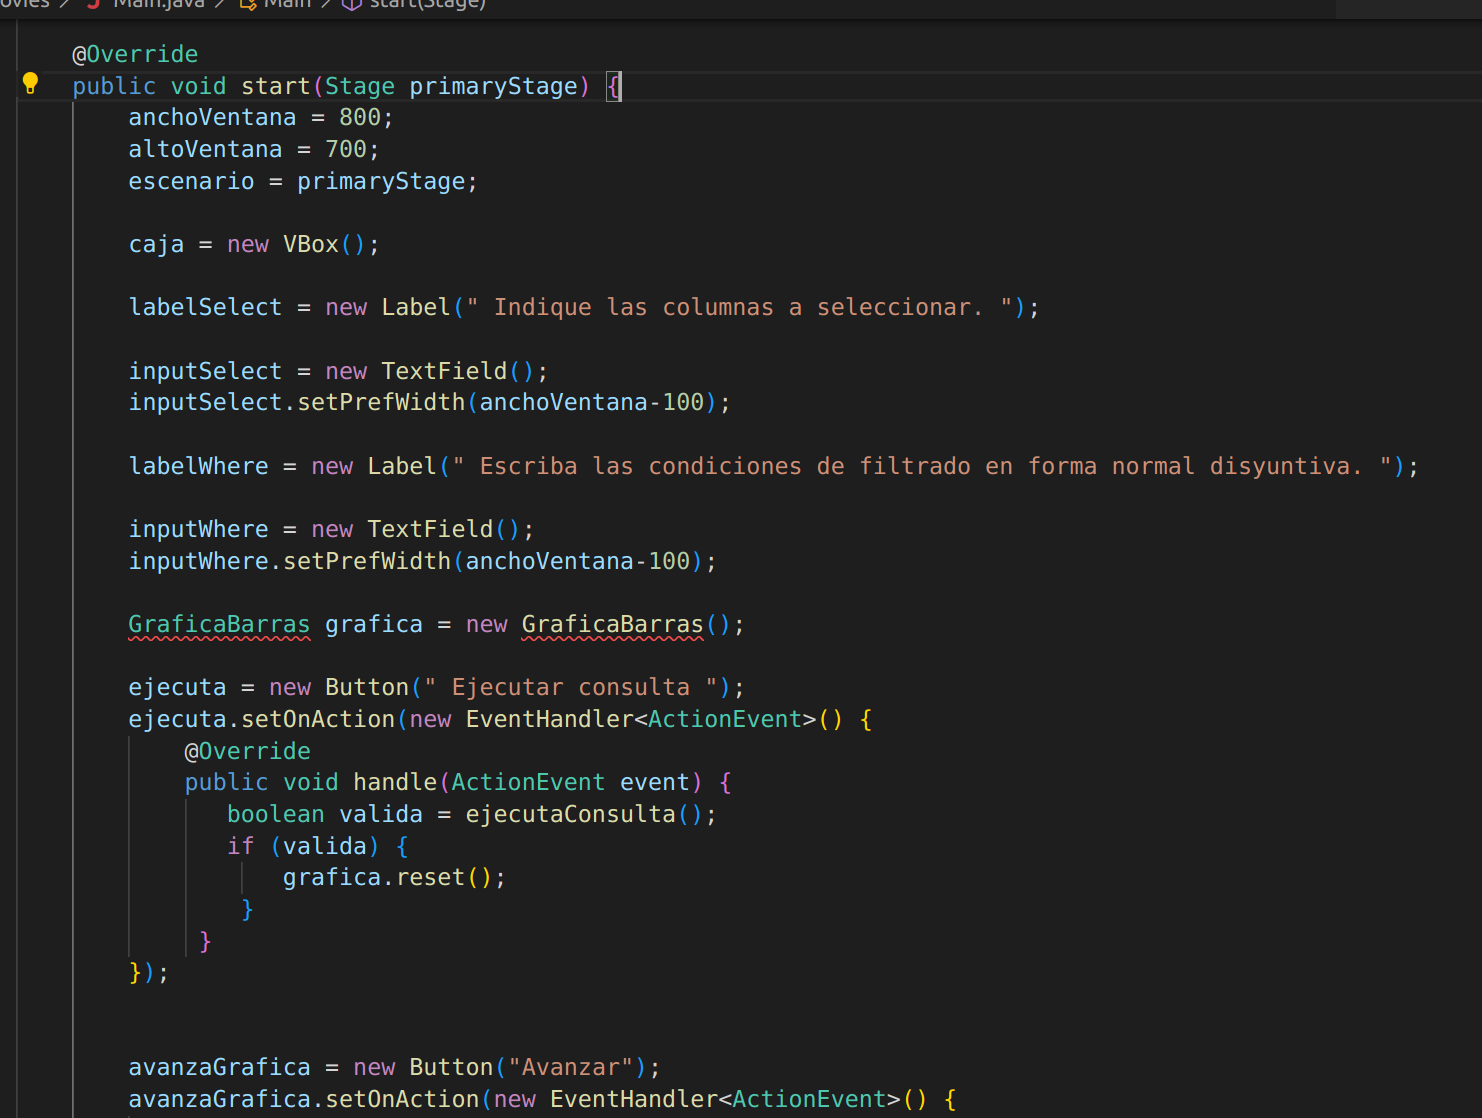
\includegraphics[width=\linewidth]{main_start1}

\end{frame}

% 2
\begin{frame}
\frametitle{Main.run}

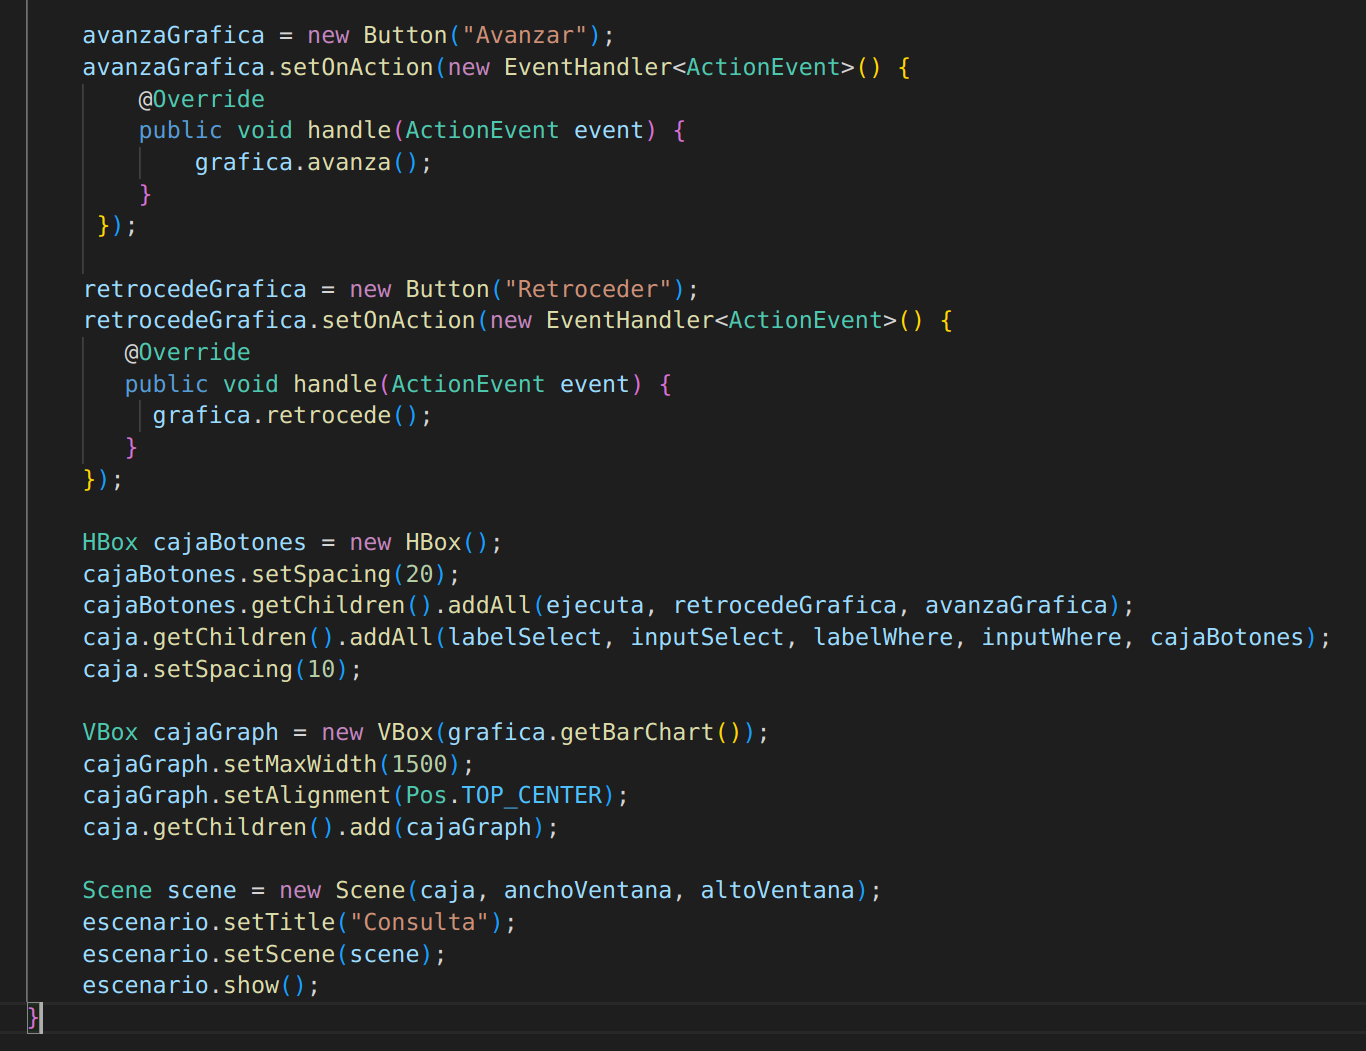
\includegraphics[width=\linewidth]{main_start2}

\end{frame}

% 3
\begin{frame}
\frametitle{Main.getNumHilos}

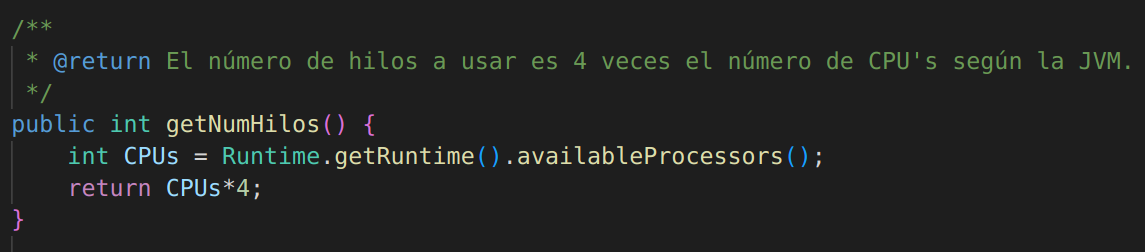
\includegraphics[width=\linewidth]{main_getnumhilos}

\end{frame}

% 4
\begin{frame}
\frametitle{Main.ejecutaConsulta}
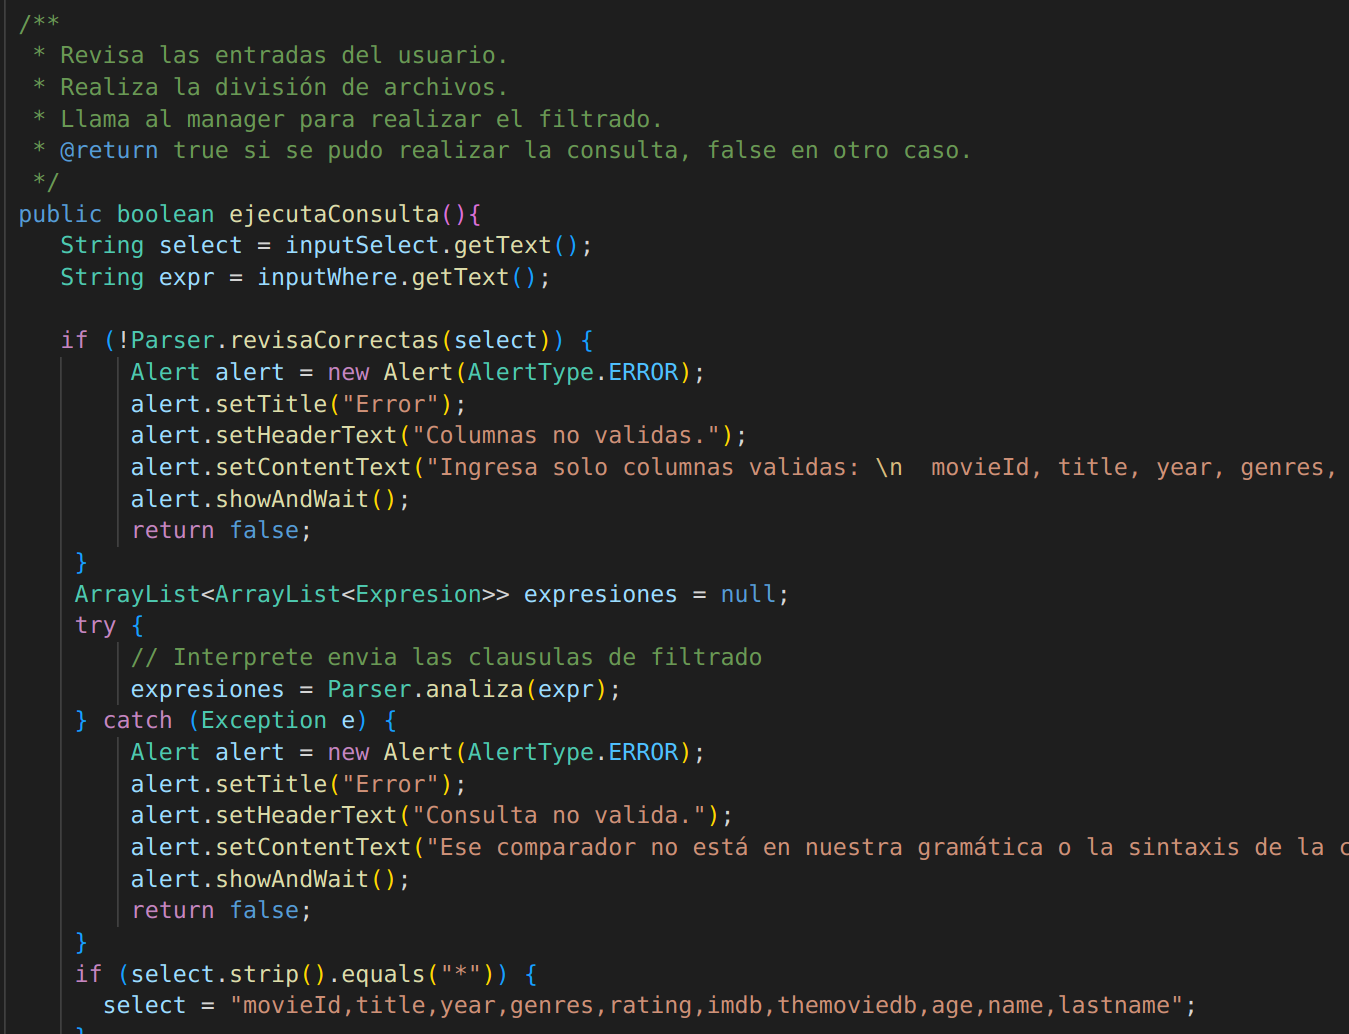
\includegraphics[width=\linewidth]{main_ejecutaconsulta1}
\end{frame}

% 5
\begin{frame}
\frametitle{Main.ejecutaConsulta}
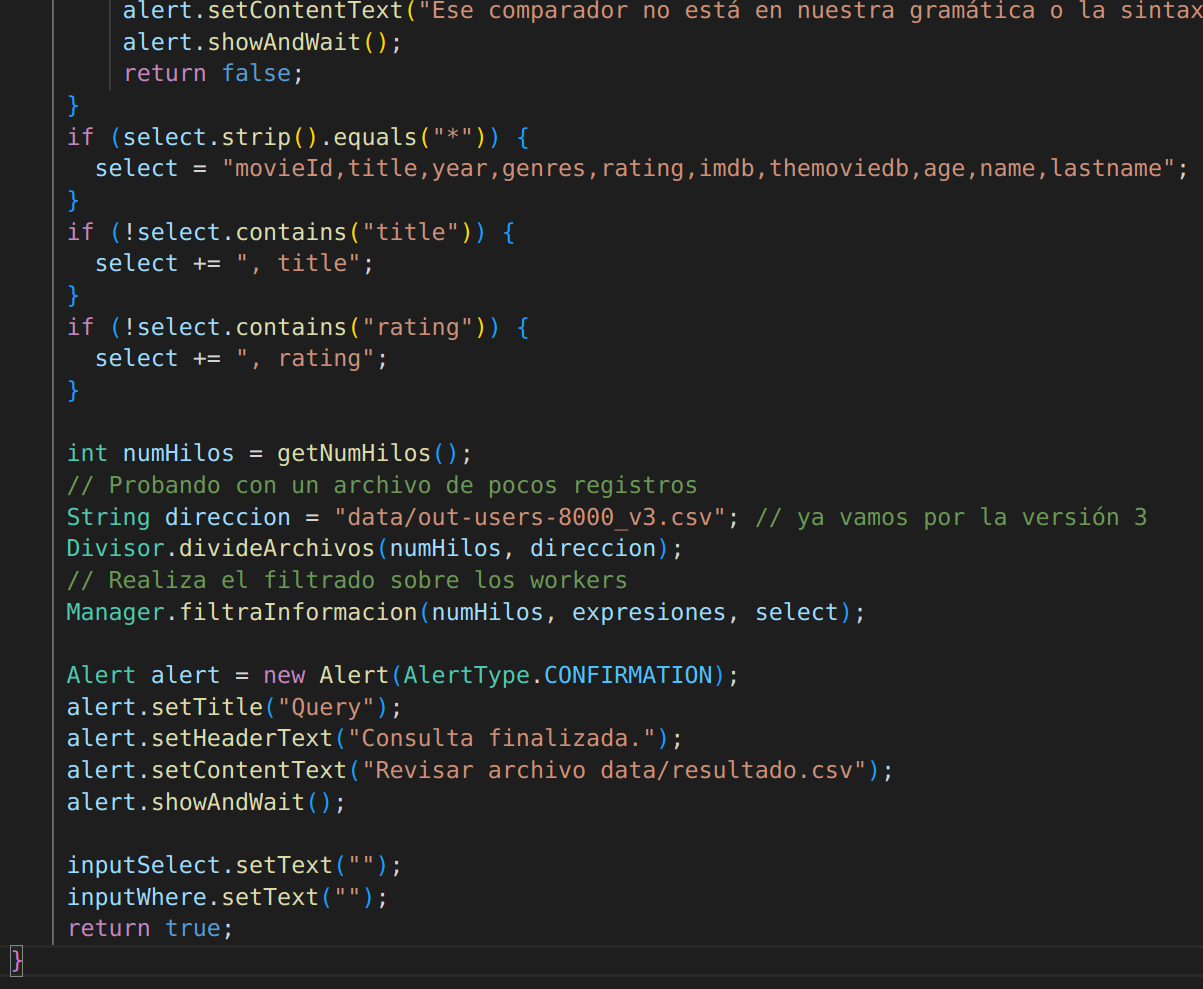
\includegraphics[width=\linewidth]{main_ejecutaconsulta2}
\end{frame}

\section{Manager}

% 6
\begin{frame}
\frametitle{Manager.filtraInformacion}
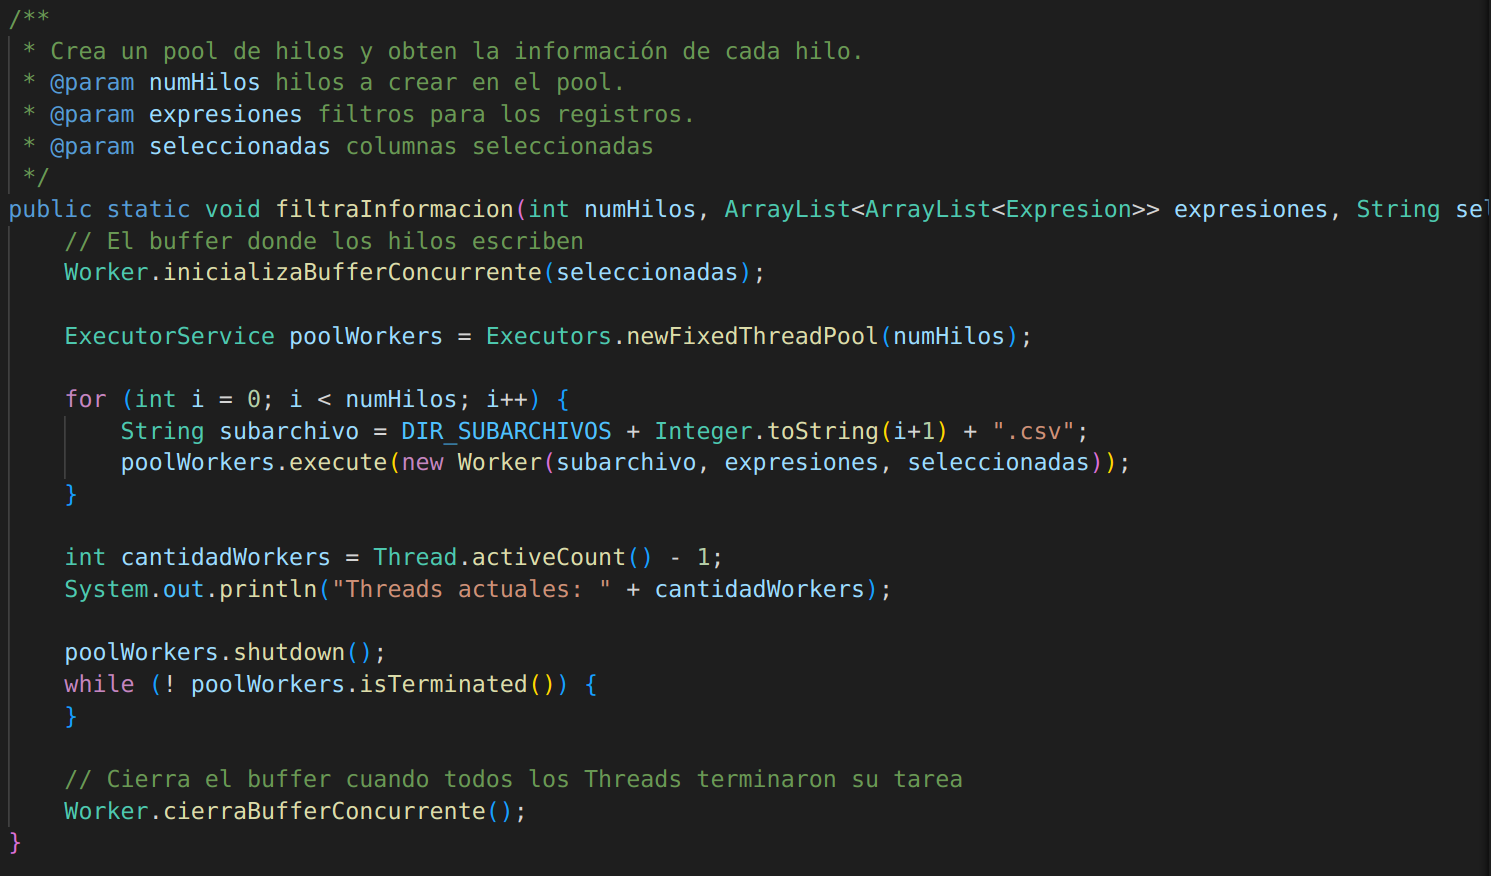
\includegraphics[width=\linewidth]{manager}
\end{frame}

\section{Worker}

% 7
\begin{frame}
\frametitle{Worker.builder}
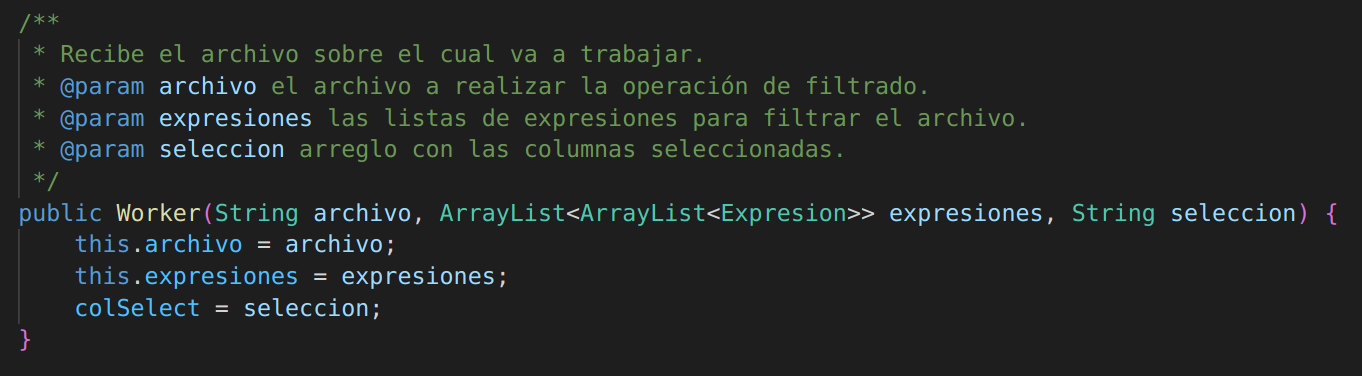
\includegraphics[width=\linewidth]{worker_builder}
\end{frame}

% 8
\begin{frame}
\frametitle{Worker.inicializaBufferConcurrente}
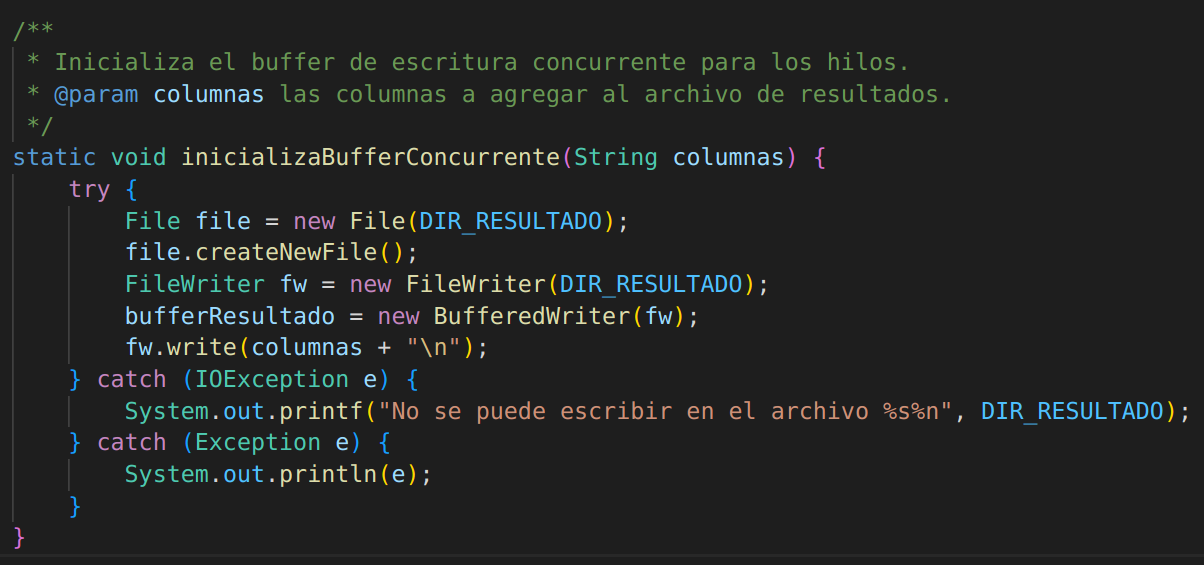
\includegraphics[width=\linewidth]{worker_inicializabufferconcurrente}
\end{frame}

% 9
\begin{frame}
\frametitle{Worker.cierraBufferConcurrente}
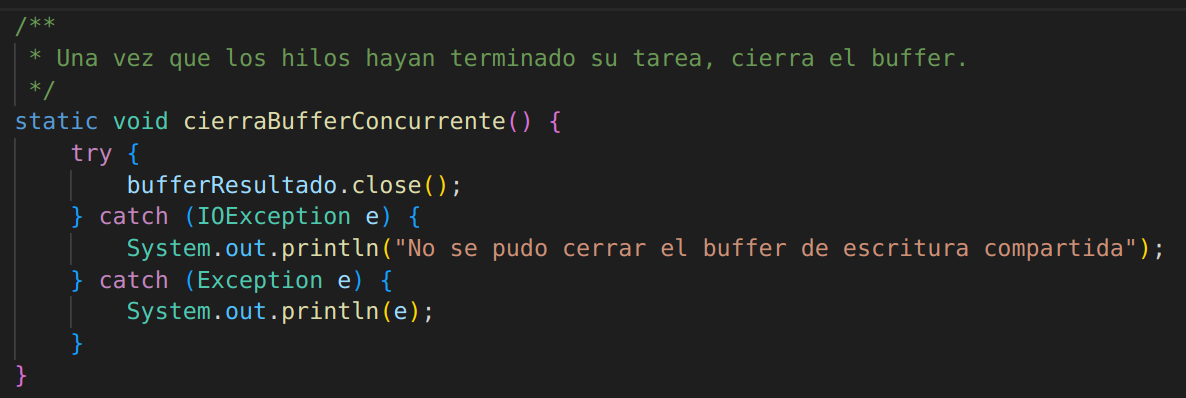
\includegraphics[width=\linewidth]{worker_cierrabufferconcurrente}
\end{frame}

% 10
\begin{frame}
\frametitle{Worker.run}
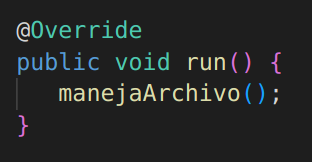
\includegraphics[width=\linewidth]{worker_run}
\end{frame}

% 11
\begin{frame}
\frametitle{Worker.seleccionaColumnas}
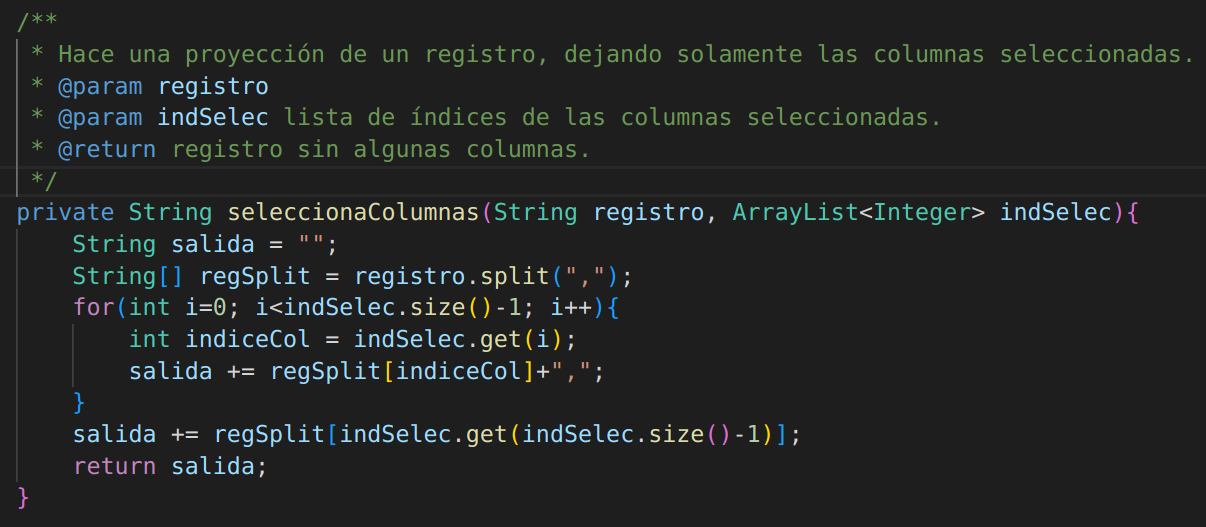
\includegraphics[width=\linewidth]{worker_seleccionacolumnas}
\end{frame}

% 12
\begin{frame}
\frametitle{Worker.manejaArchivo}
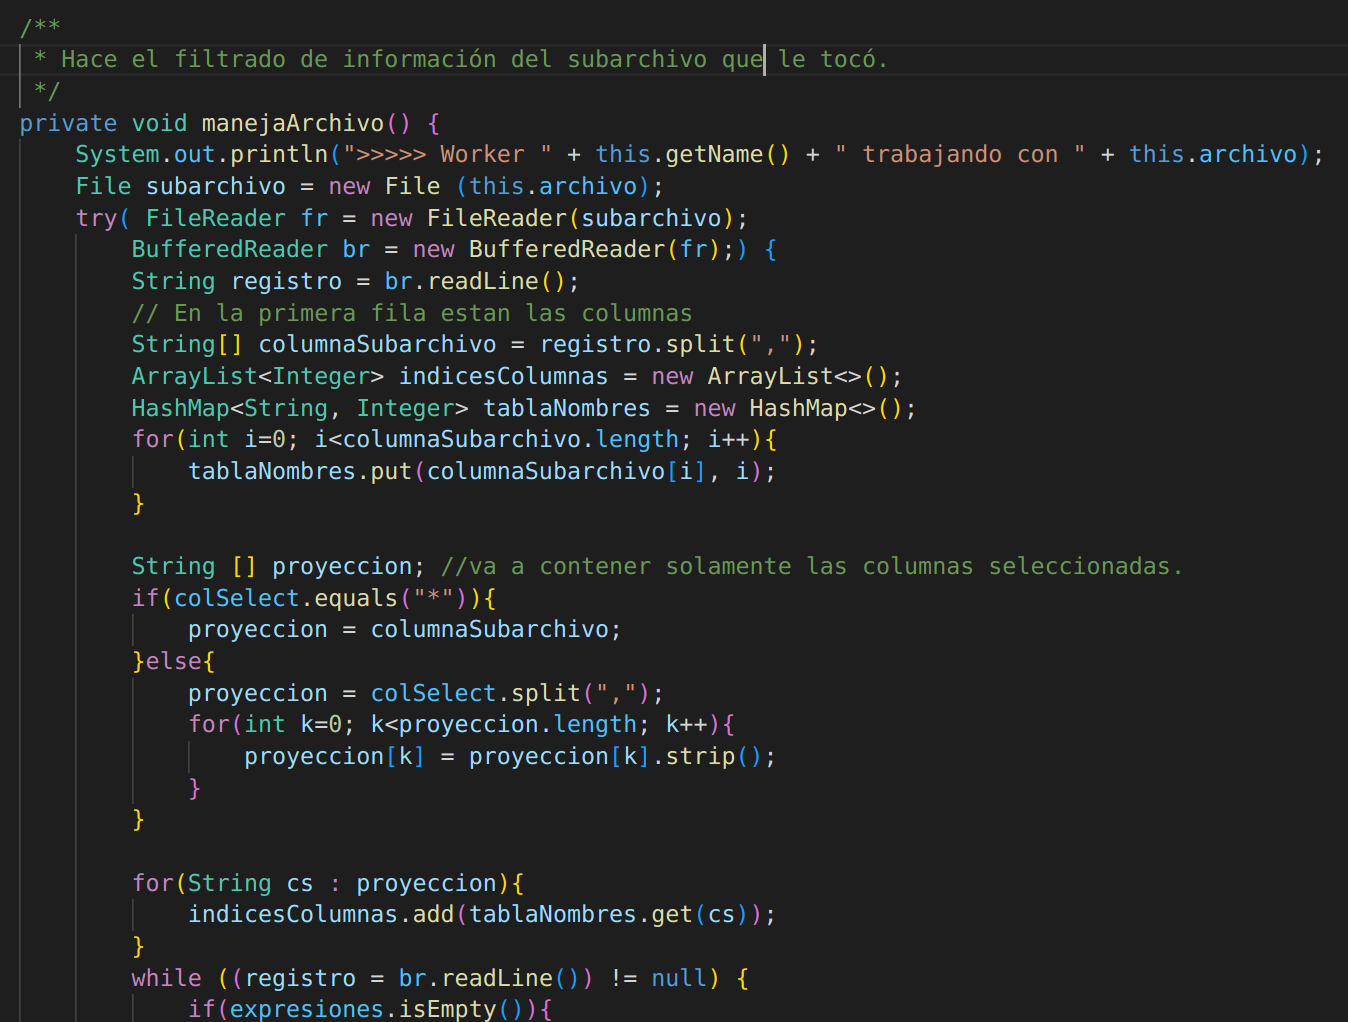
\includegraphics[width=\linewidth]{worker_manejaarchivo1}
\end{frame}

% 13
\begin{frame}
\frametitle{Worker.manejaArchivo}
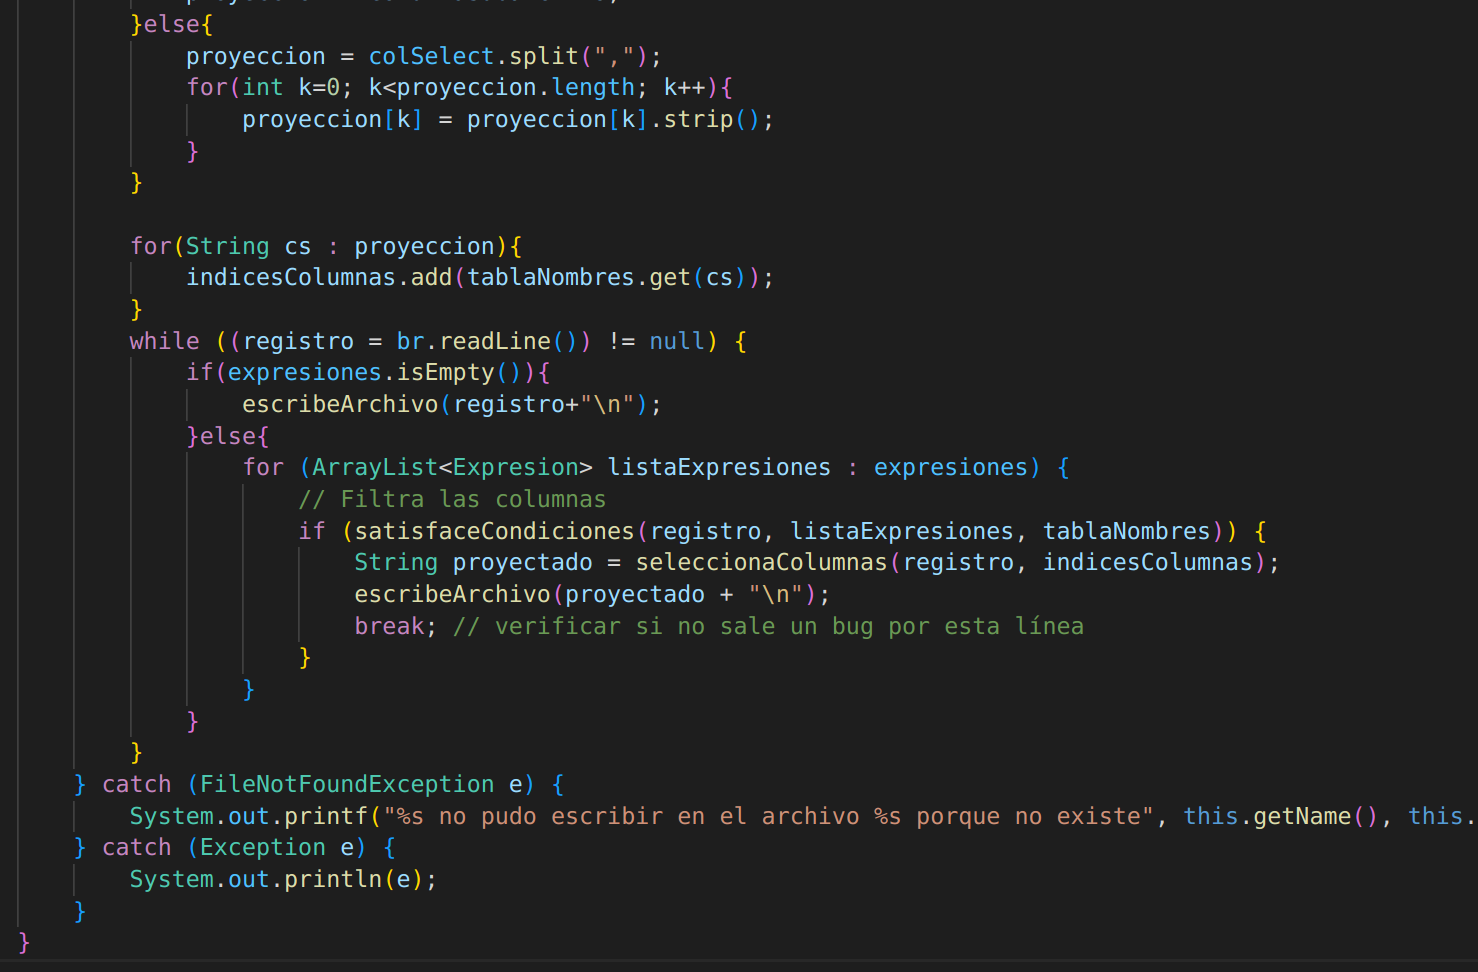
\includegraphics[width=\linewidth]{worker_manejaarchivo2}
\end{frame}

% 14
\begin{frame}
\frametitle{Worker.escribeArchivo}
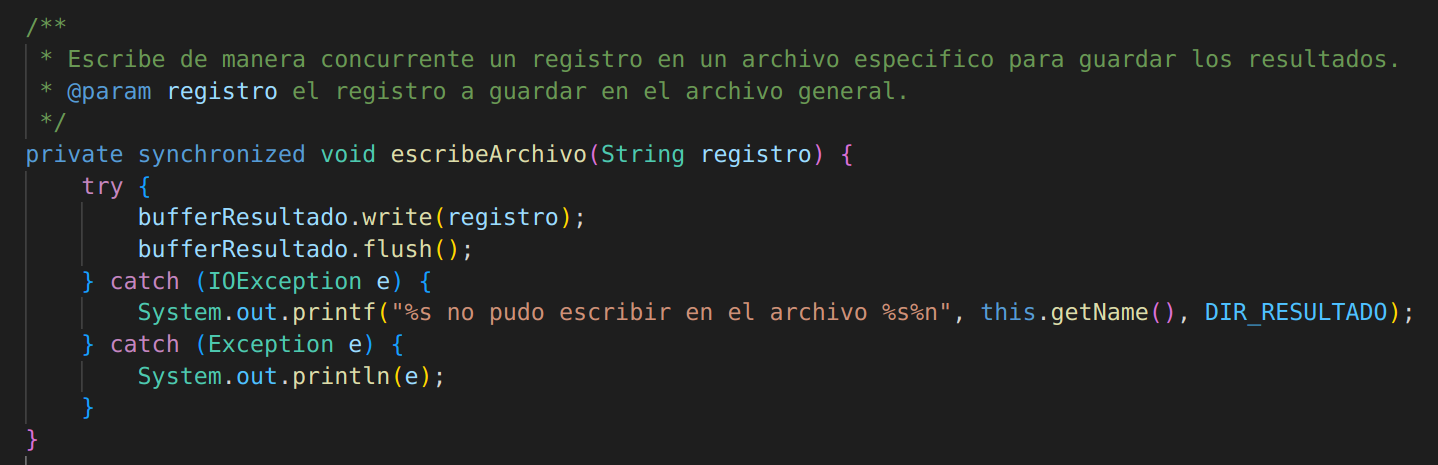
\includegraphics[width=\linewidth]{worker_escribearchivo}
\end{frame}

% 15
\begin{frame}
\frametitle{Worker.tipoColumna}
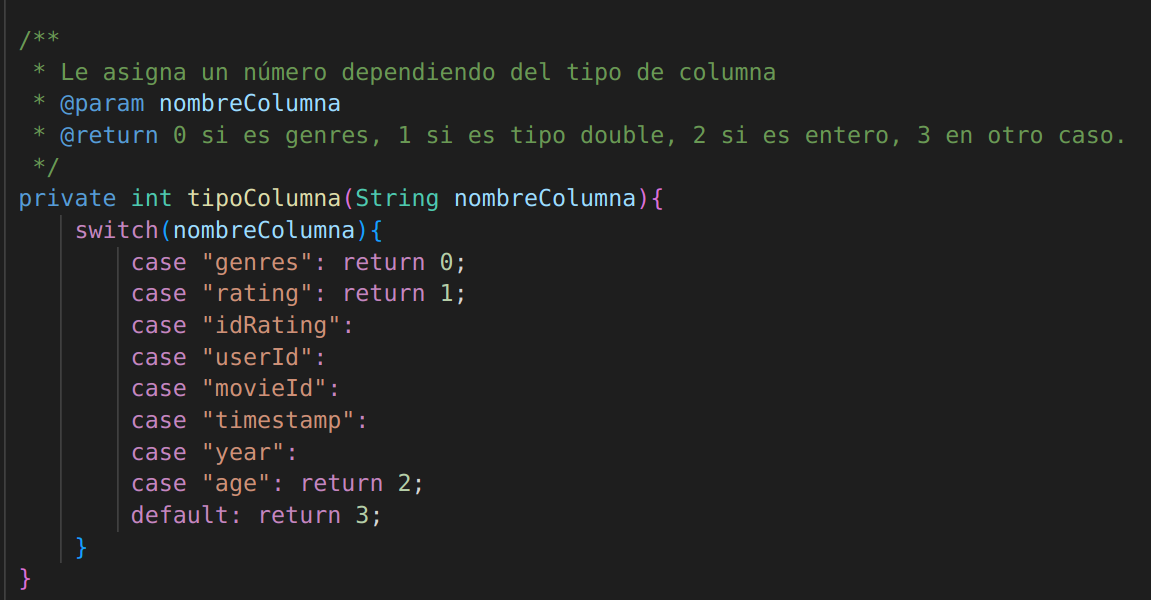
\includegraphics[width=\linewidth]{worker_tipocolumna}
\end{frame}

% 16
\begin{frame}
\frametitle{Worker.satisfaceCondiciones}
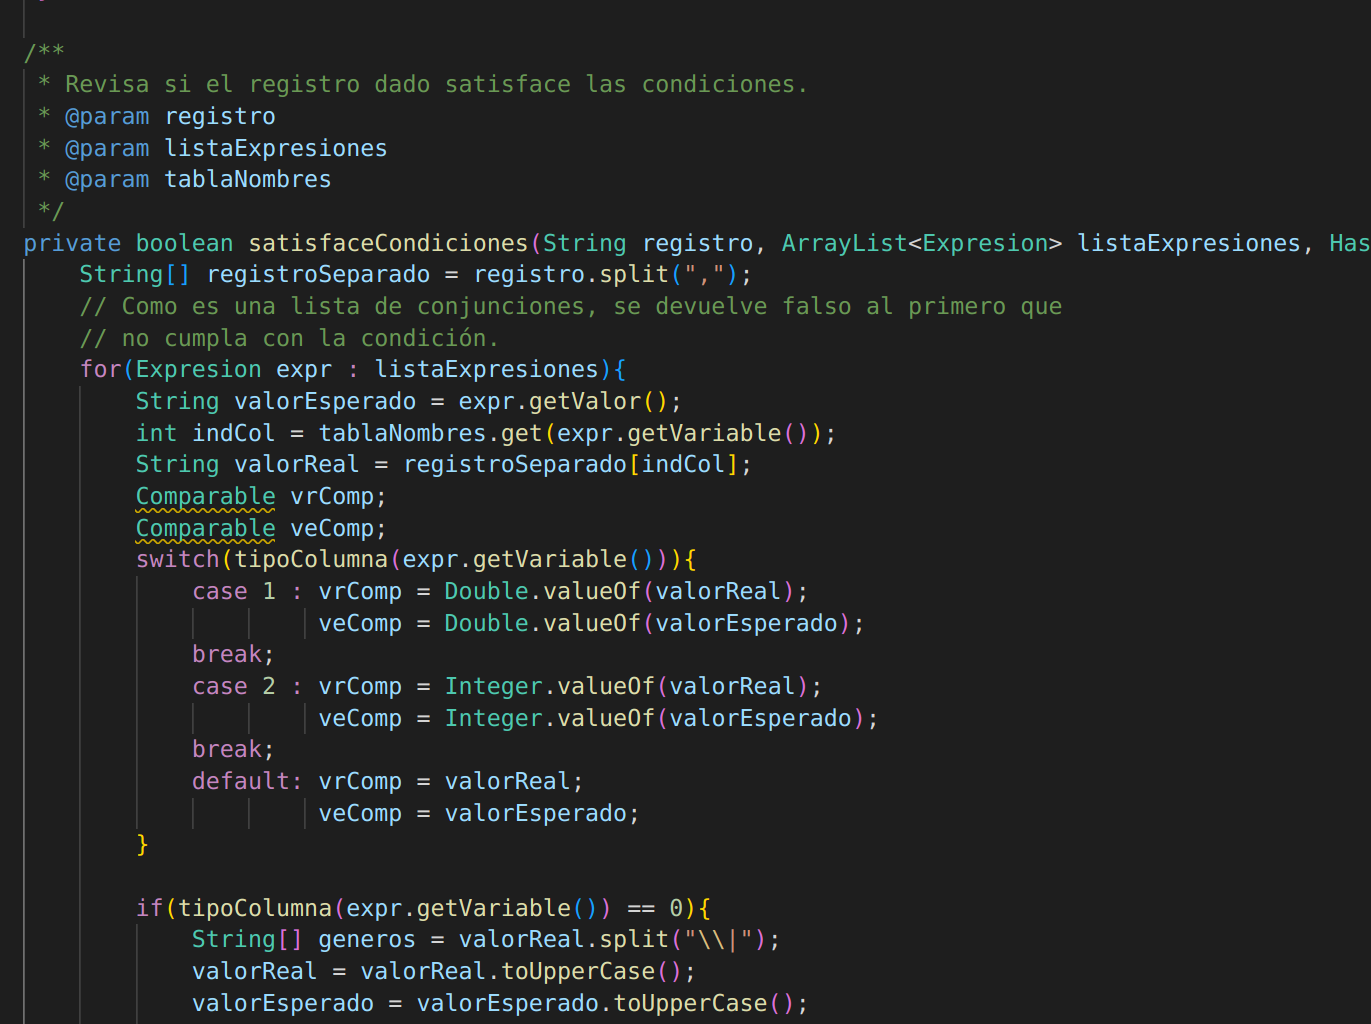
\includegraphics[width=0.9\linewidth]{worker_satisfacecondiciones1}
\end{frame}

% 17
\begin{frame}
\frametitle{Worker.satisfaceCondiciones}
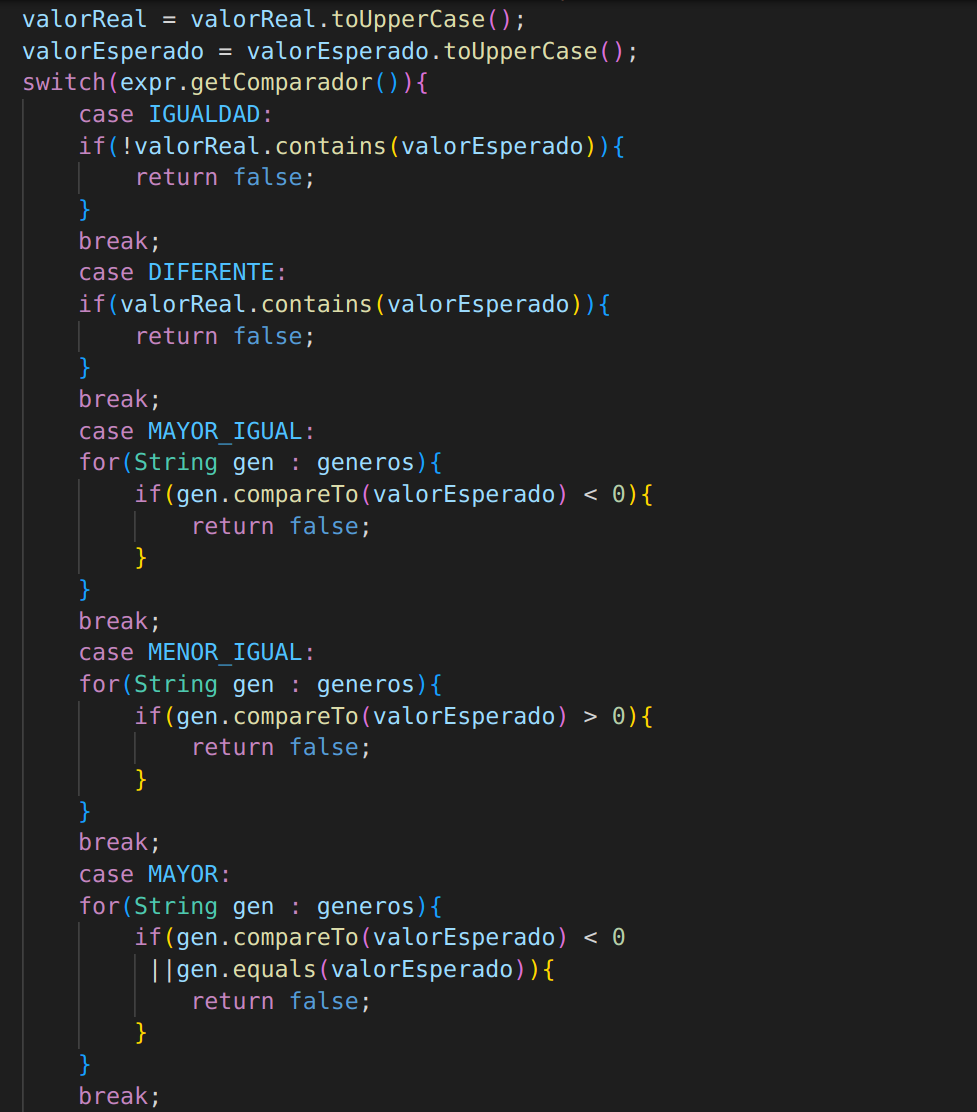
\includegraphics[width=0.7\linewidth]{worker_satisfacecondiciones2}
\end{frame}

% 18
\begin{frame}
\frametitle{Worker.satisfaceCondiciones}
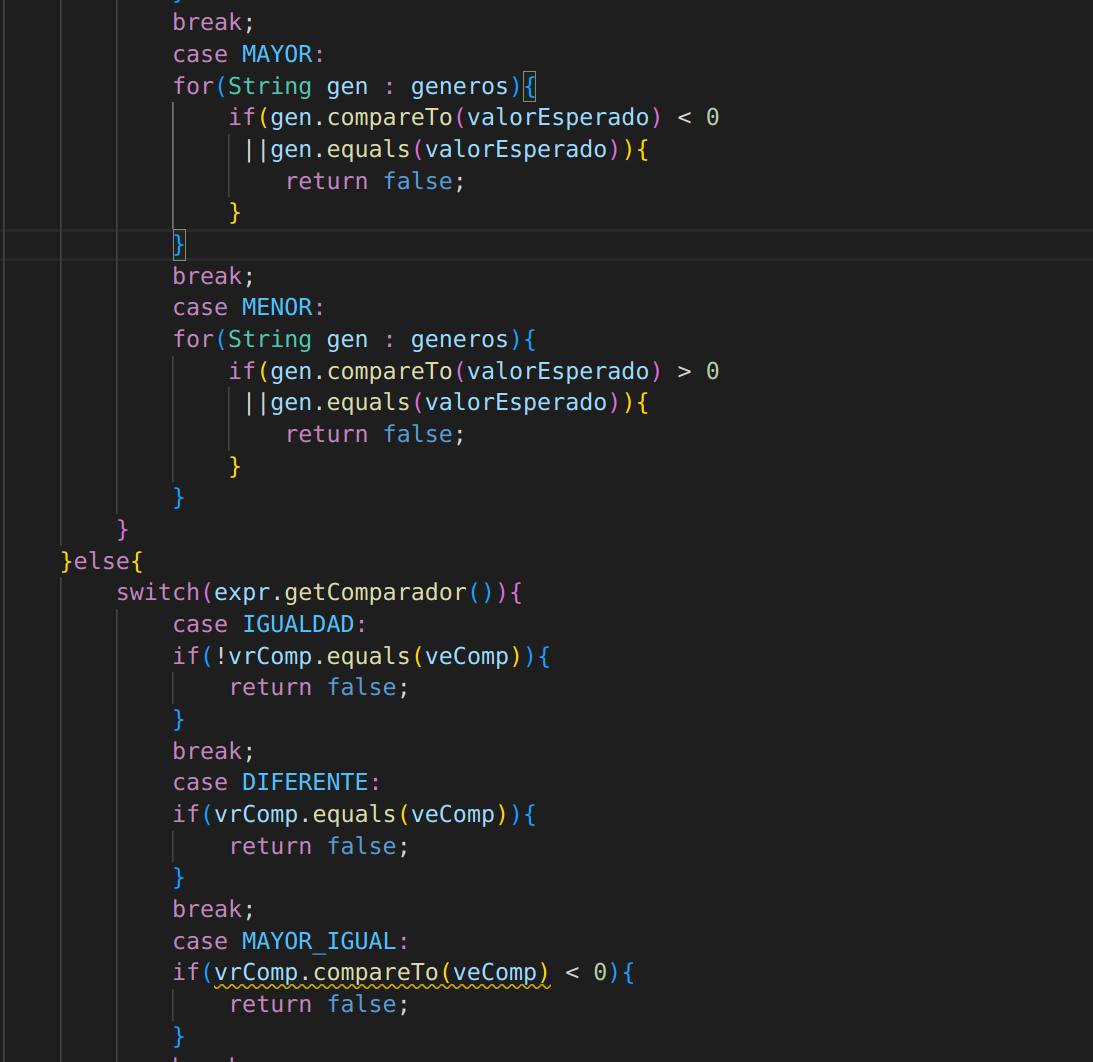
\includegraphics[width=0.9\linewidth]{worker_satisfacecondiciones3}
\end{frame}

% 19
\begin{frame}
\frametitle{Worker.satisfaceCondiciones}
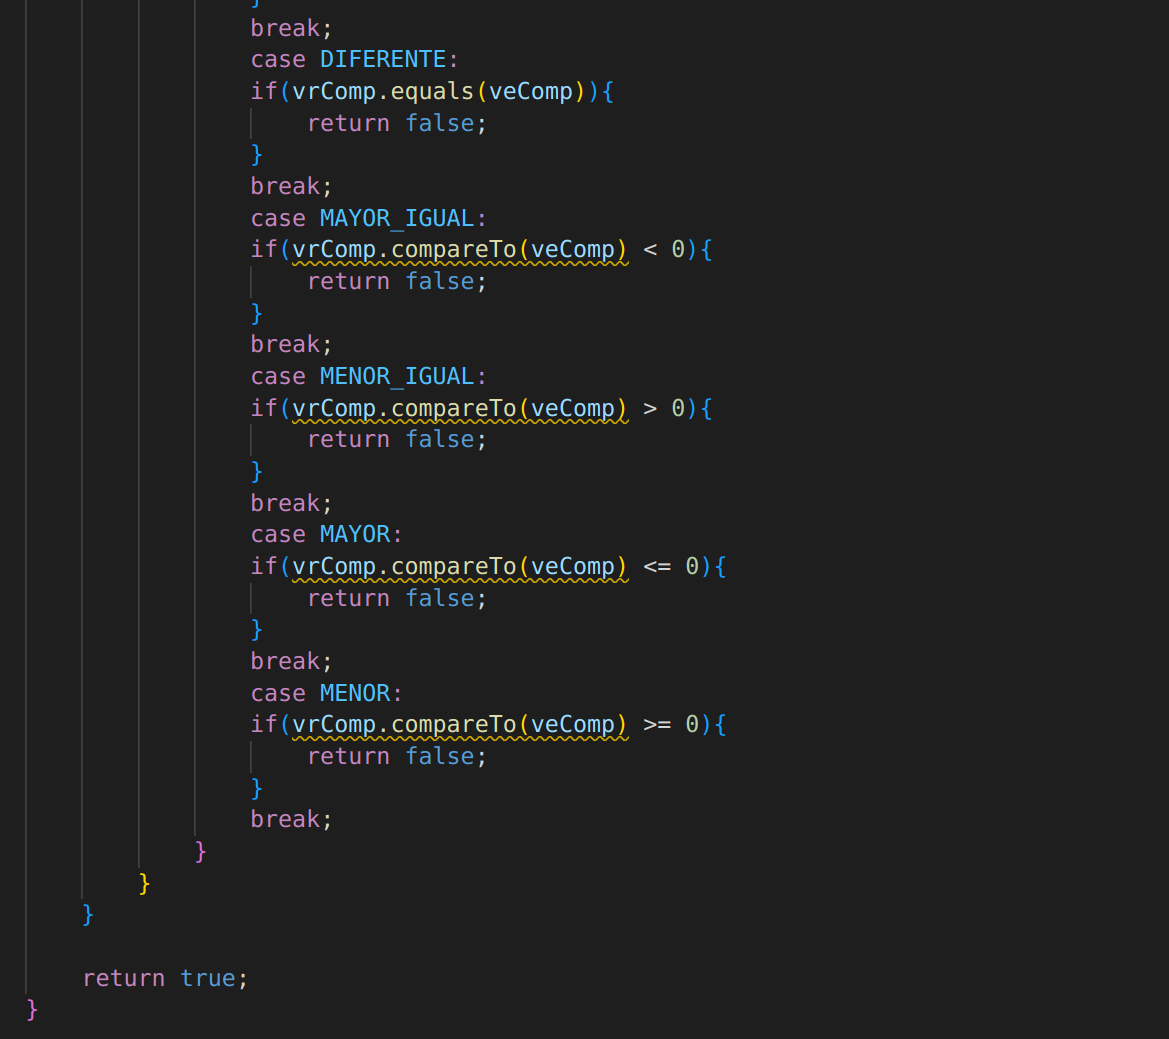
\includegraphics[width=0.9\linewidth]{worker_satisfacecondiciones4}
\end{frame}

\section{ComparadorEnum}

% 20
\begin{frame}
\frametitle{ComparadorEnum}
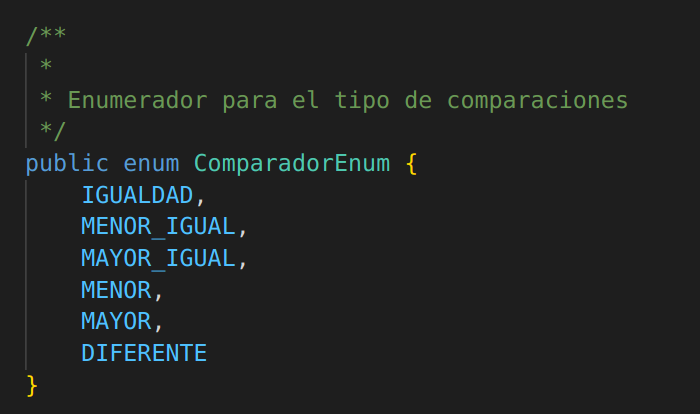
\includegraphics[width=\linewidth]{comparadorenum}
\end{frame}

\section{Divisor}

% 21
\begin{frame}
\frametitle{Divisor.divideArchivos}
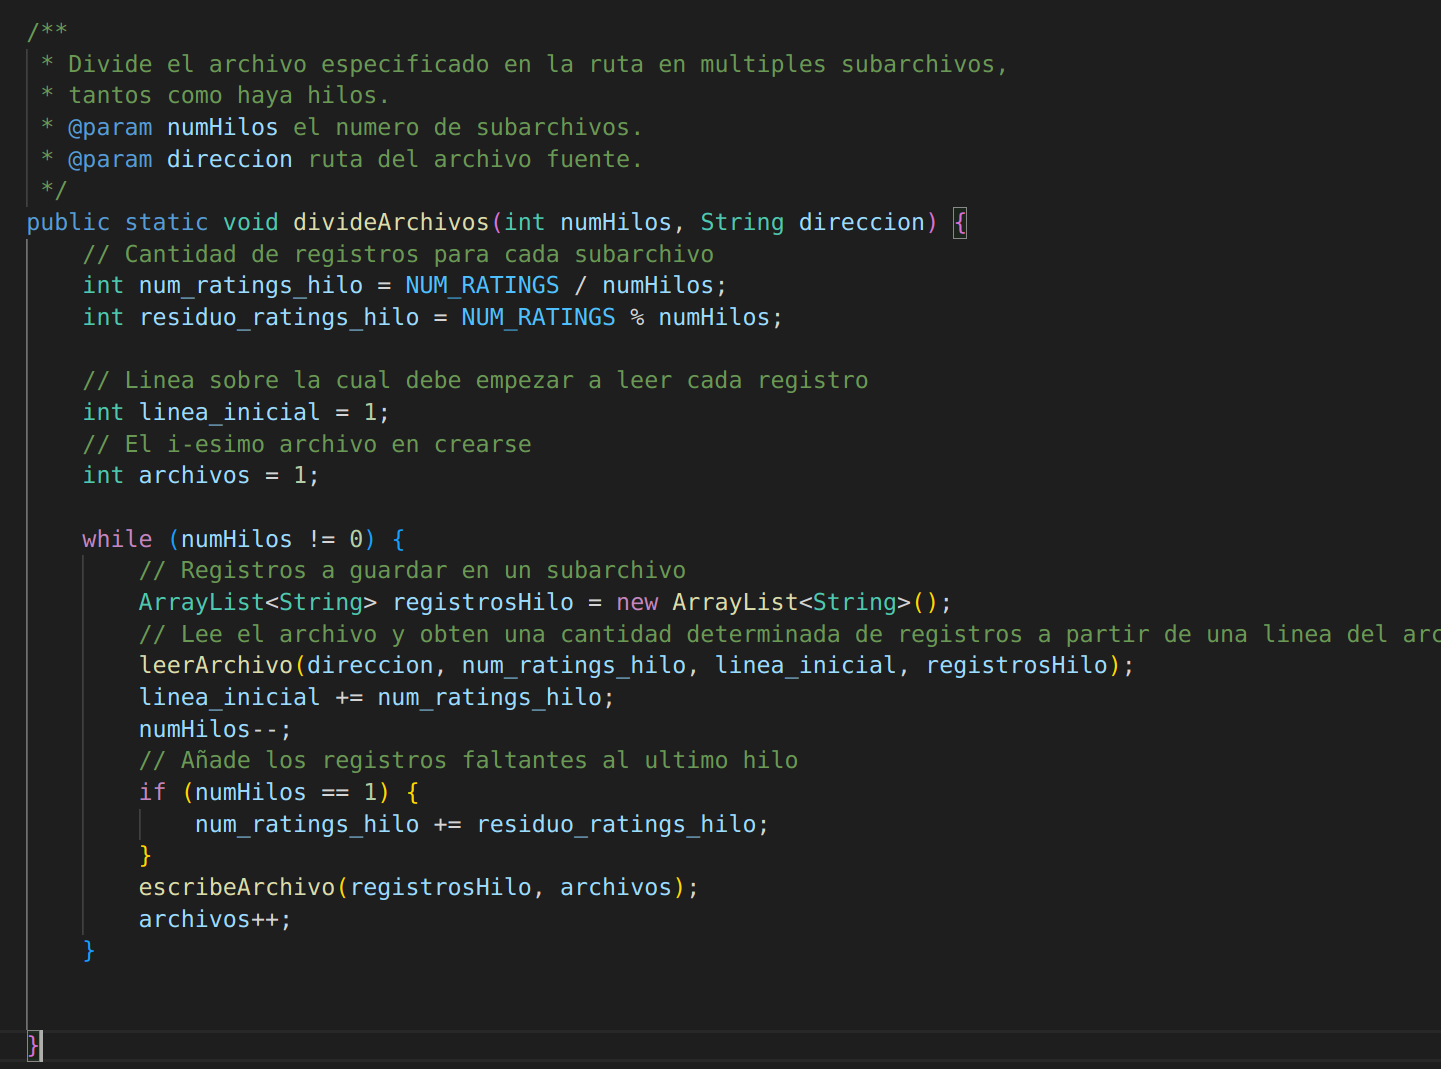
\includegraphics[width=\linewidth]{divisor_dividearchivos}
\end{frame}

% 22
\begin{frame}
\frametitle{Divisor.leeArchivo}
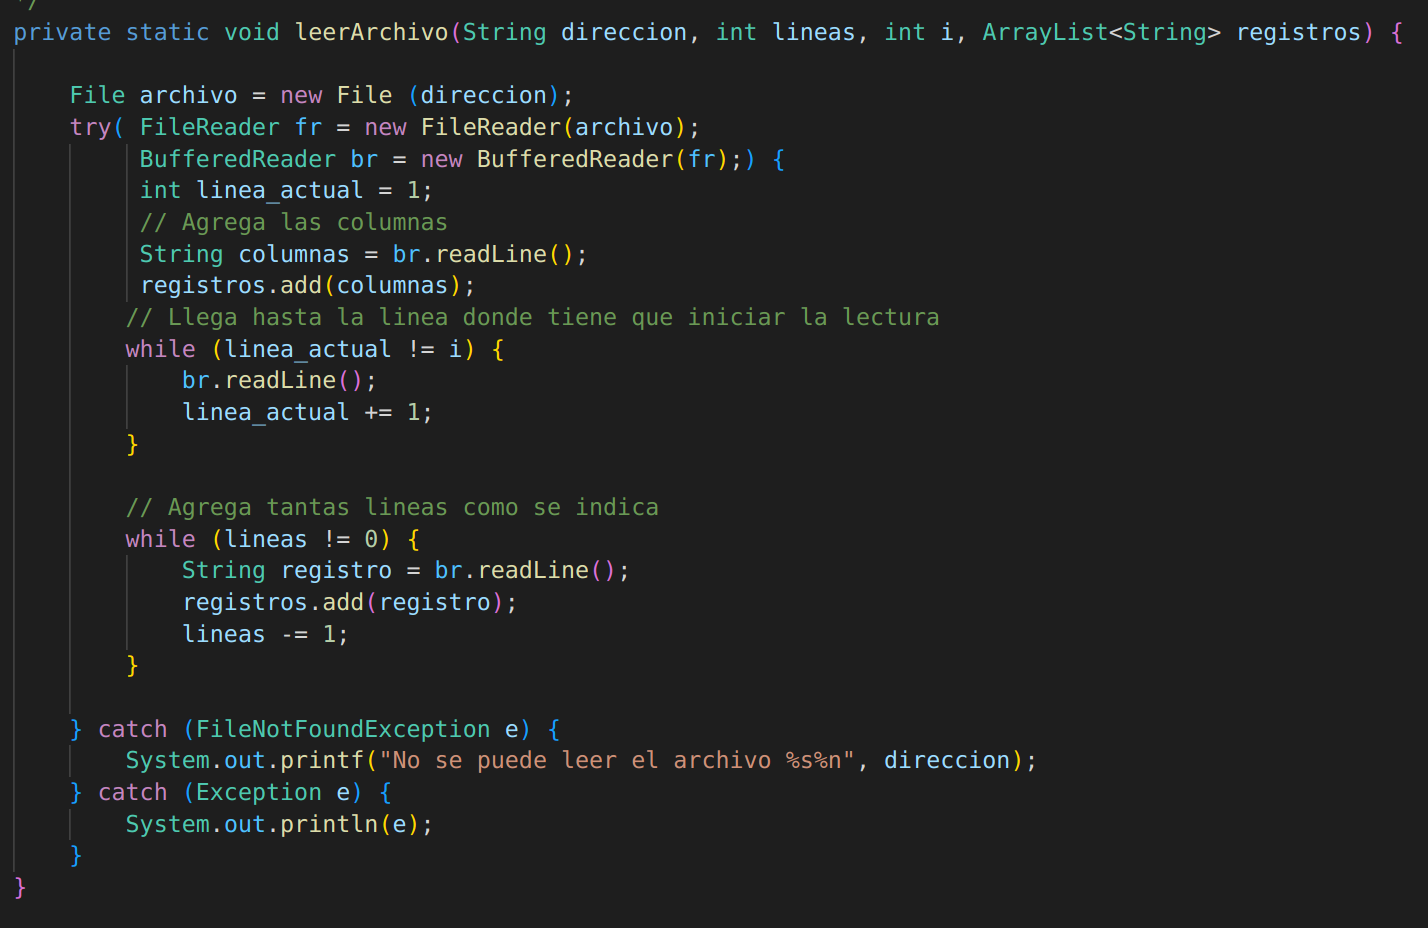
\includegraphics[width=\linewidth]{divisor_leearchivo}
\end{frame}

% 23
\begin{frame}
\frametitle{Divisor.escribeArchivo}
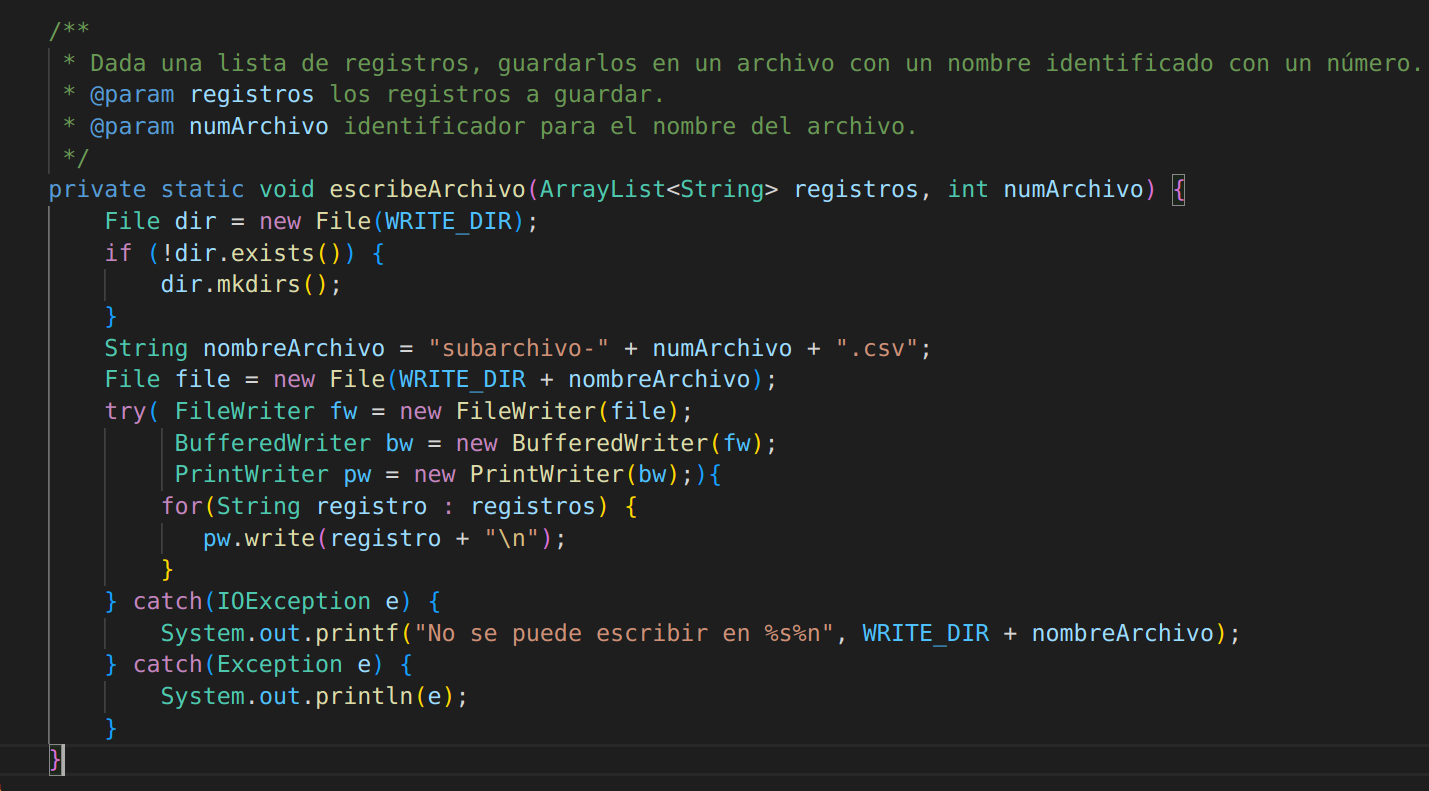
\includegraphics[width=\linewidth]{divisor_escribearchivo}
\end{frame}

\section{Expresion}

% 24
\begin{frame}
\frametitle{Expresion.builder}
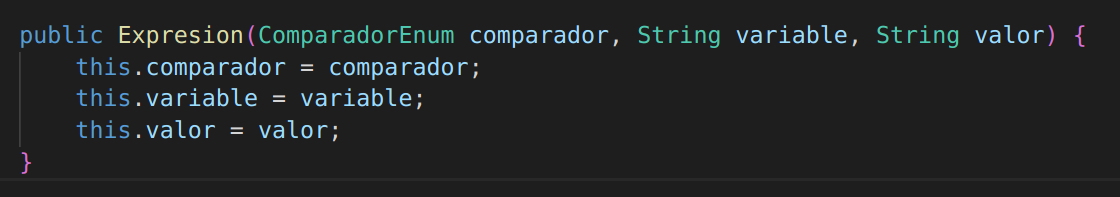
\includegraphics[width=\linewidth]{expresion_builder}
\end{frame}

\section{Parser}

% 25
\begin{frame}
\frametitle{Parser.splitConector}
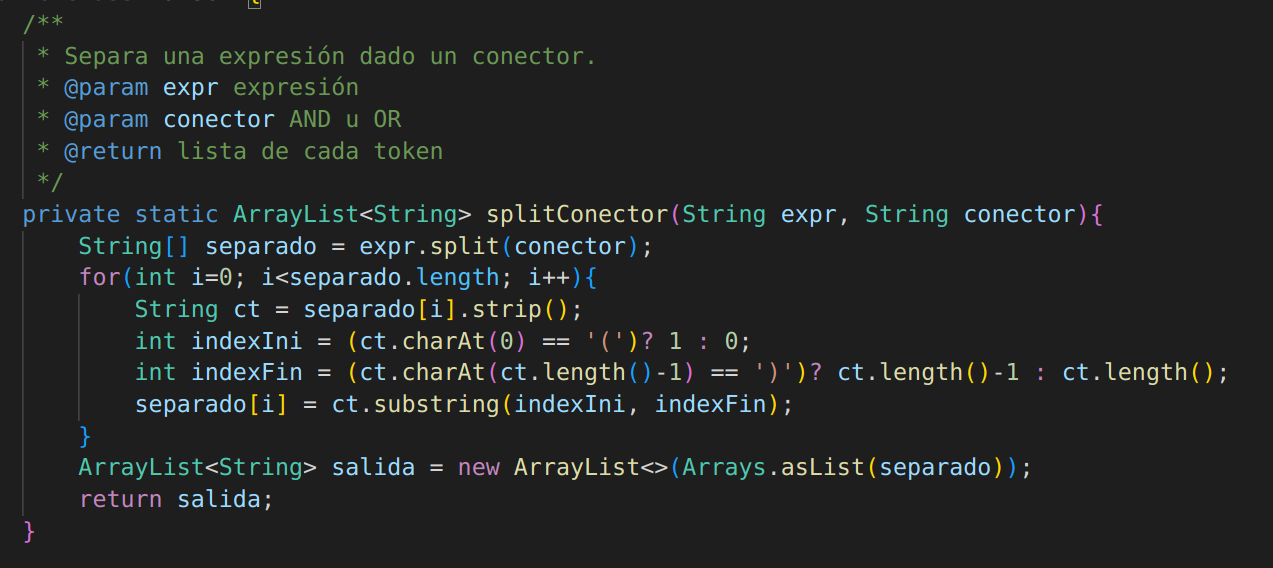
\includegraphics[width=\linewidth]{parser_splitconector}
\end{frame}

% 26
\begin{frame}
\frametitle{Parser.fnd}
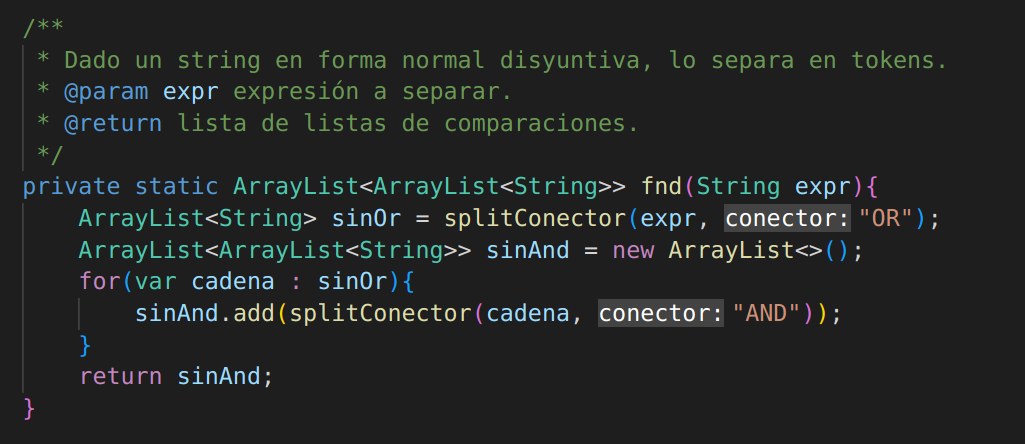
\includegraphics[width=\linewidth]{parser_fnd}
\end{frame}

% 27
\begin{frame}
\frametitle{Parser.extraeOperador}
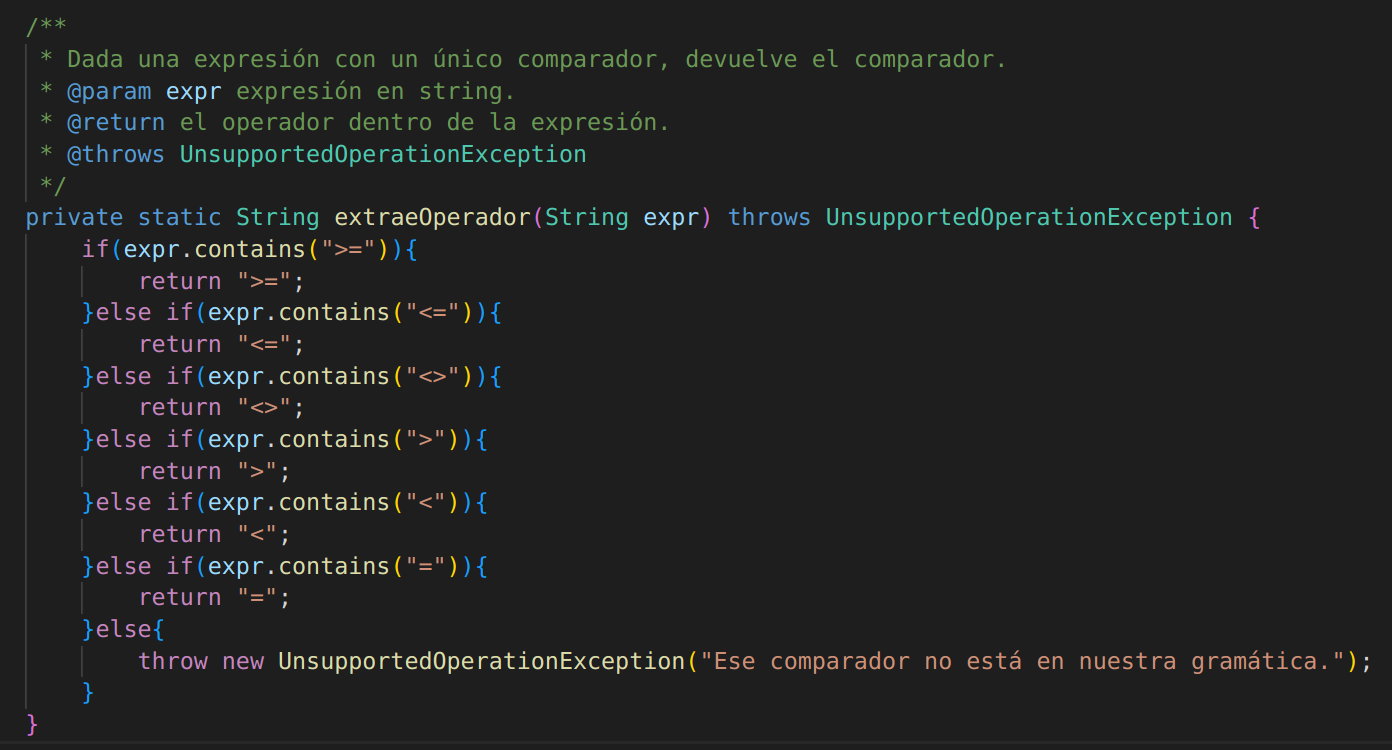
\includegraphics[width=\linewidth]{parser_extraeoperador}
\end{frame}

% 28
\begin{frame}
\frametitle{Parser.buildExpr}
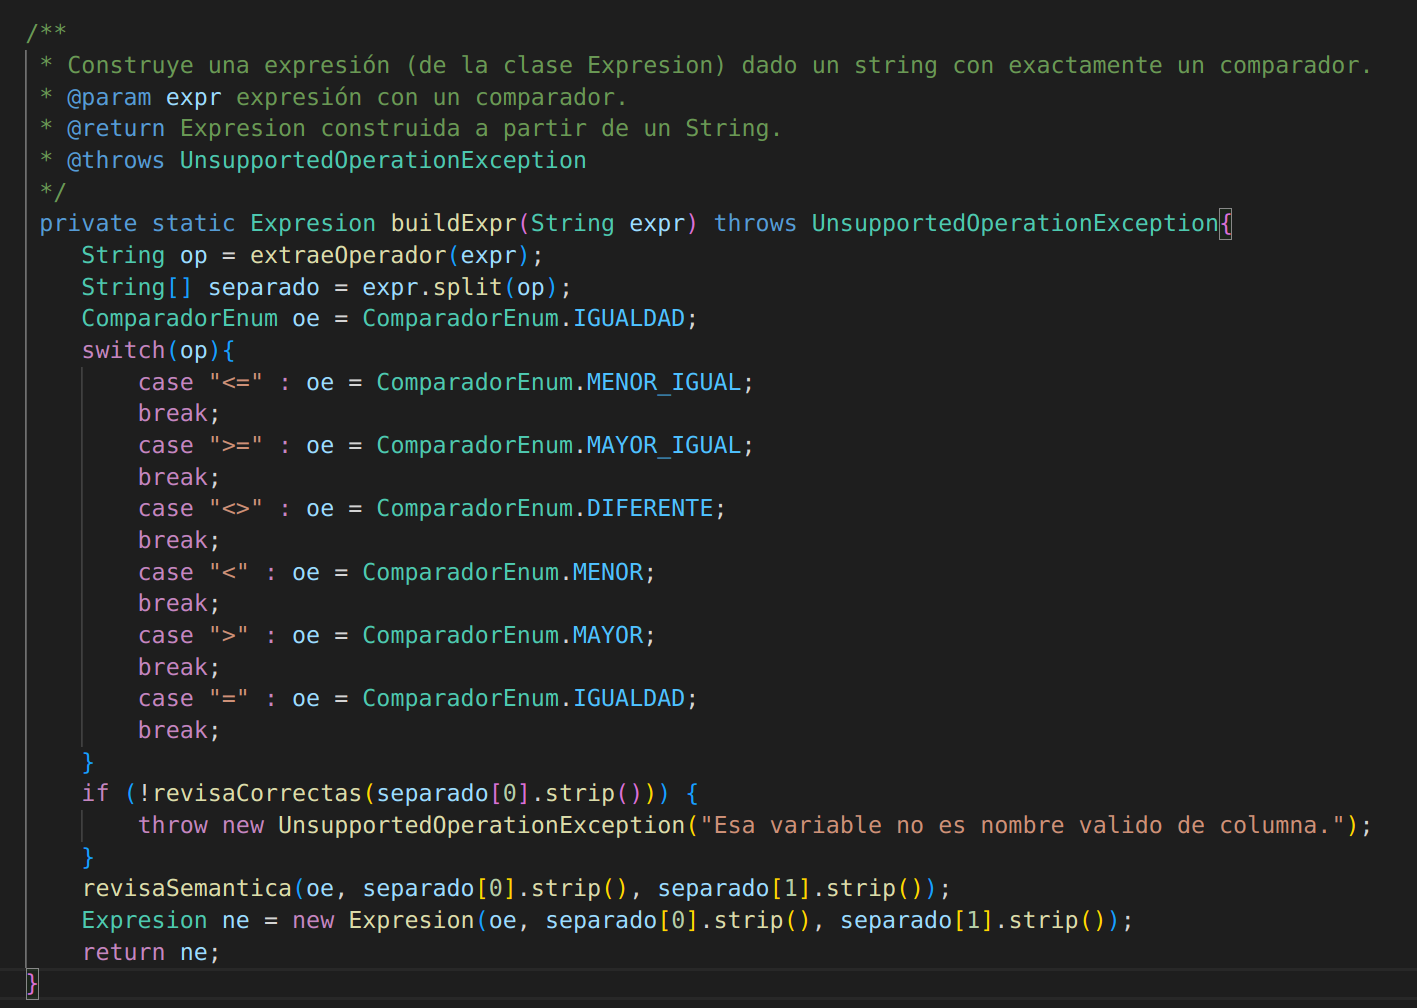
\includegraphics[width=\linewidth]{parser_buildexpr}
\end{frame}

% 29
\begin{frame}
\frametitle{Parser.revisaSemantica}
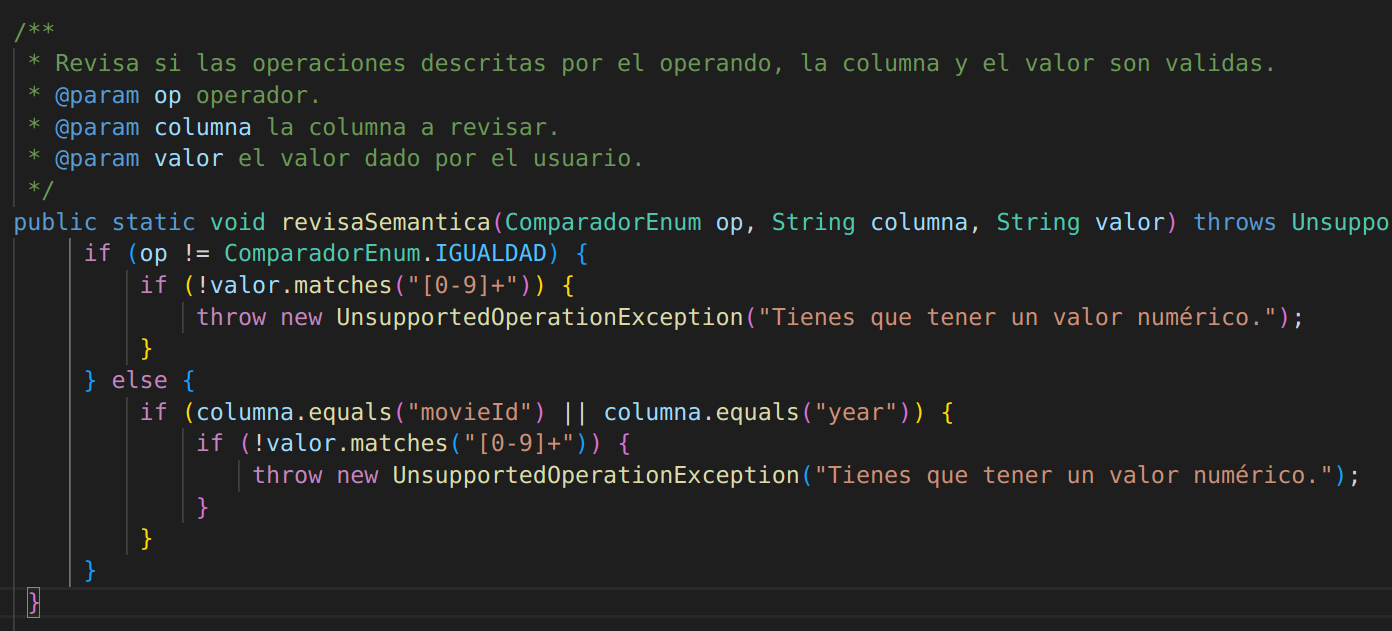
\includegraphics[width=\linewidth]{parser_revisasemantica}
\end{frame}

% 30
\begin{frame}
\frametitle{Parser.analiza}
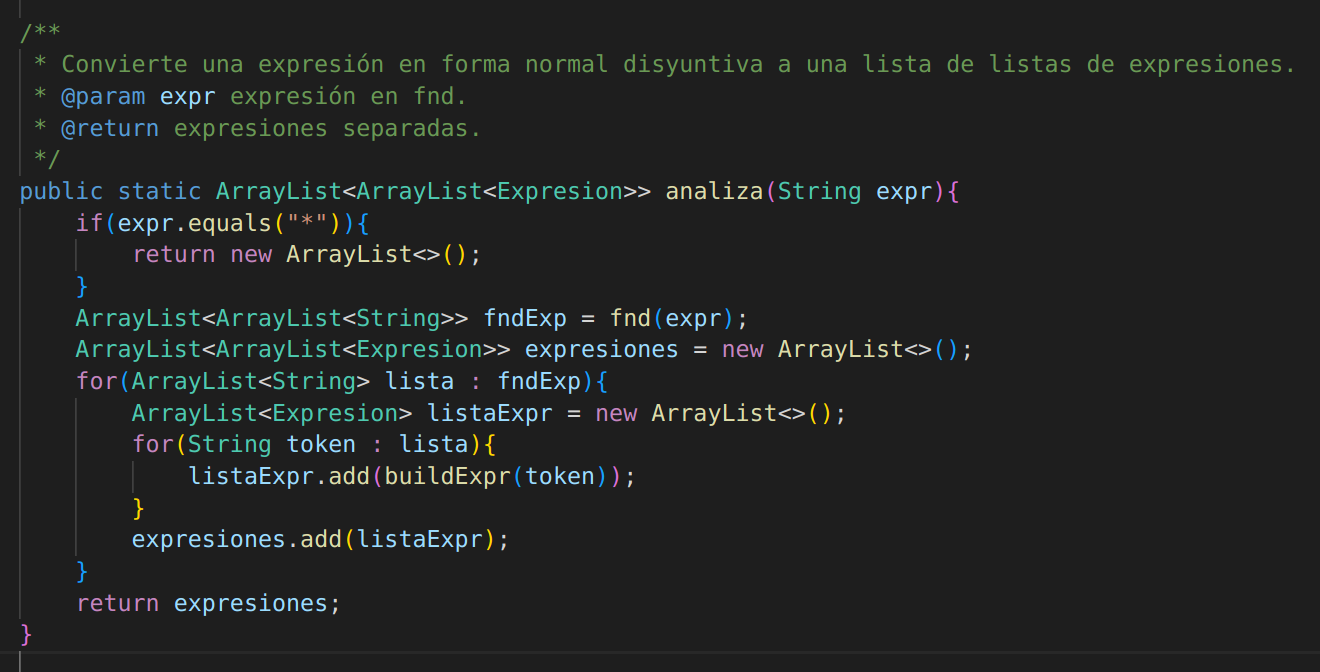
\includegraphics[width=\linewidth]{parser_analiza}
\end{frame}

% 31
\begin{frame}
\frametitle{Parser.revisaCorrectas}
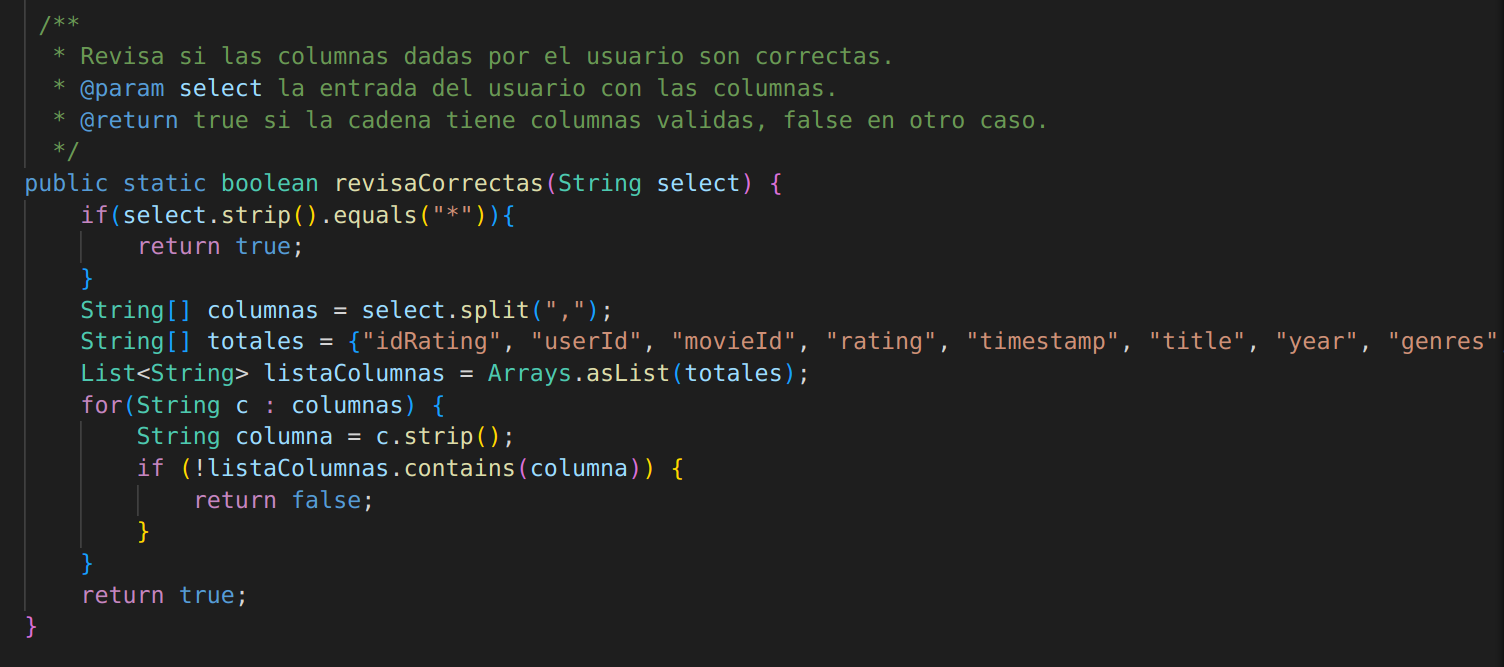
\includegraphics[width=\linewidth]{parser_revisacorrectas}
\end{frame}

\section{EstadisticaRating}

% 32
\begin{frame}
\frametitle{EstadisticaRating}
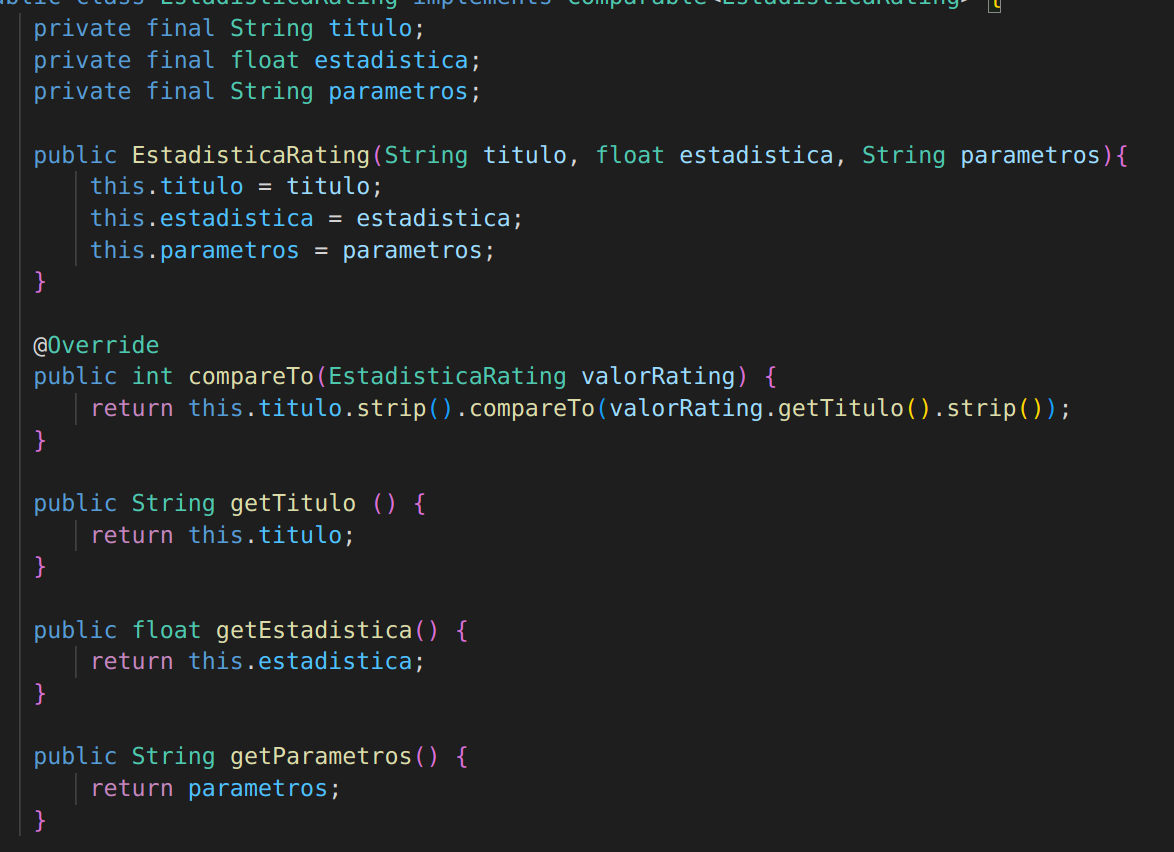
\includegraphics[width=\linewidth]{estadisticarating}
\end{frame}

% 33
\begin{frame}
\frametitle{GeneraEstadisticas.estadisticasRatingPromedio}
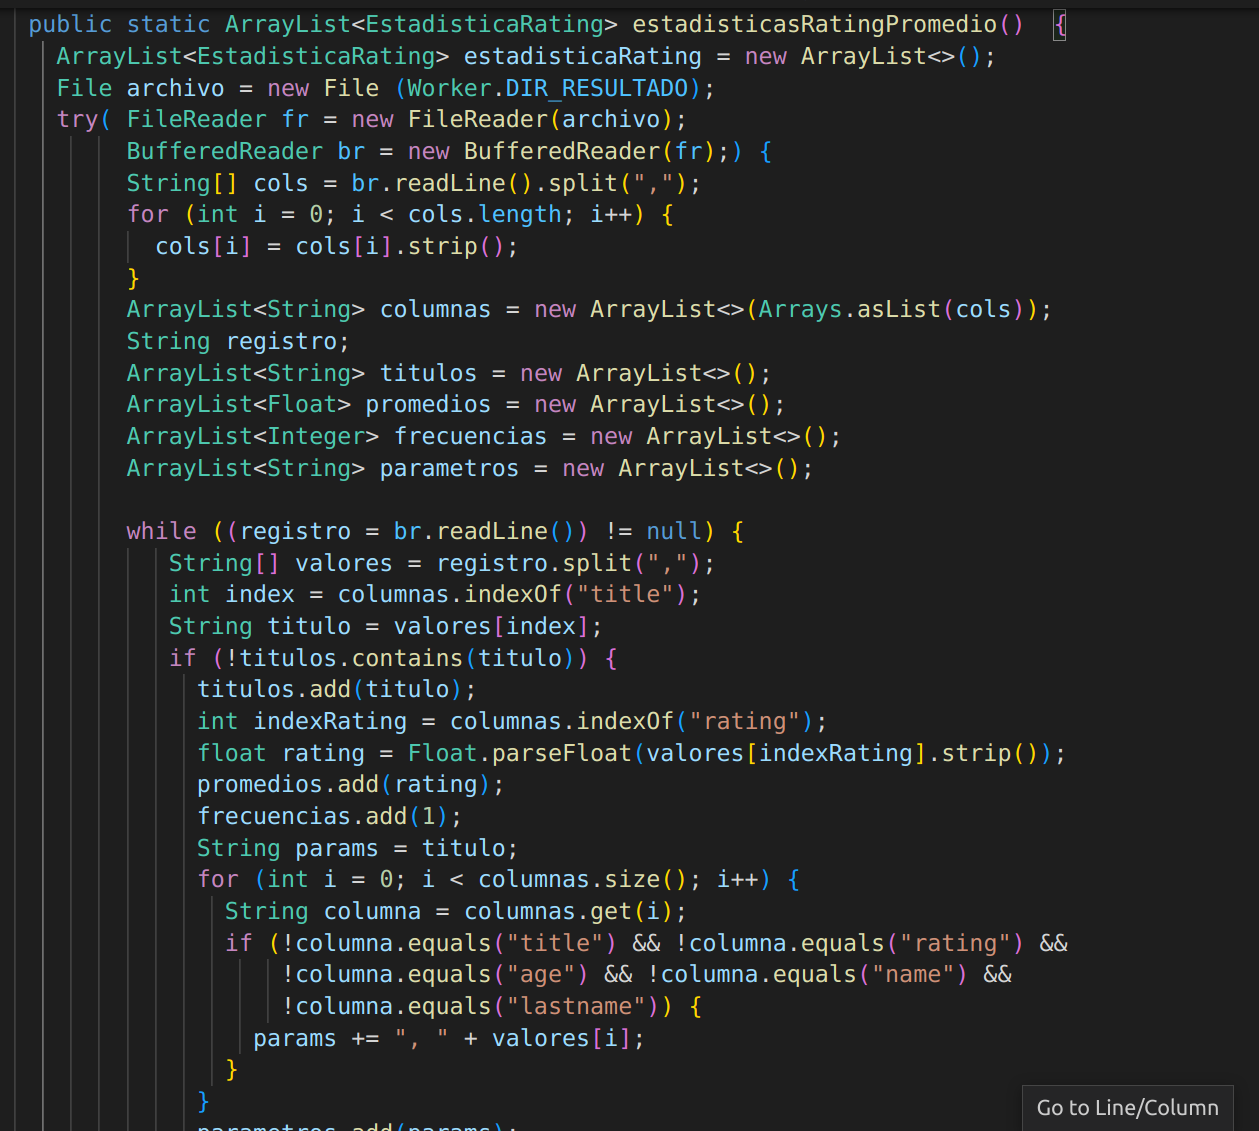
\includegraphics[width=0.9\linewidth]{generaestadisticas_estadisticasratingpromedio1}
\end{frame}

% 34
\begin{frame}
\frametitle{GeneraEstadisticas.estadisticasRatingPromedio}
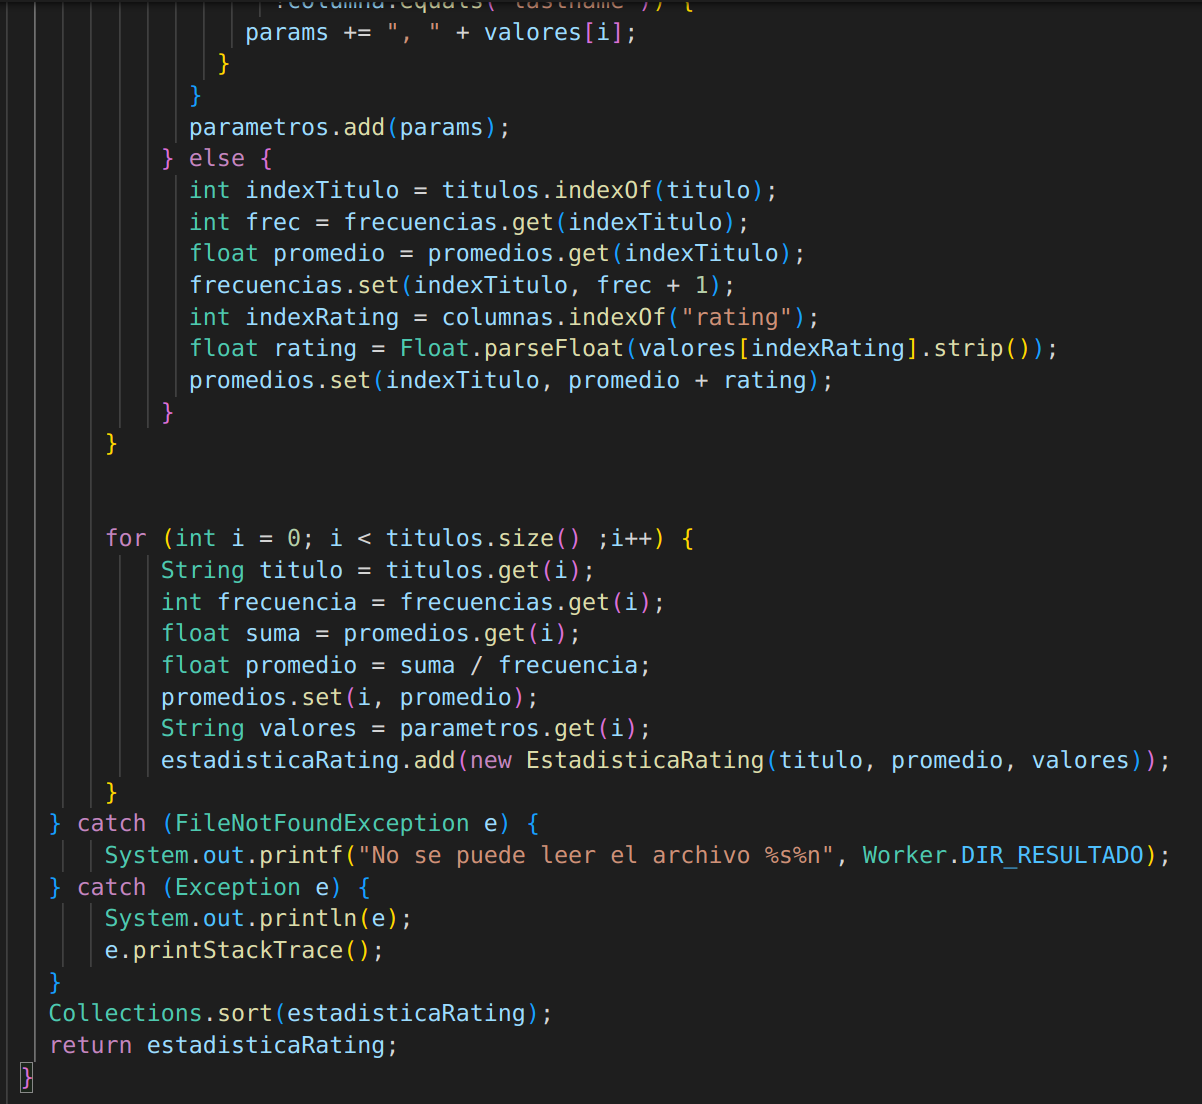
\includegraphics[width=0.9\linewidth]{generaestadisticas_estadisticasratingpromedio2}
\end{frame}

% 35
\begin{frame}
\frametitle{GeneraEstadisticas.estadisticasRatingMinimo}
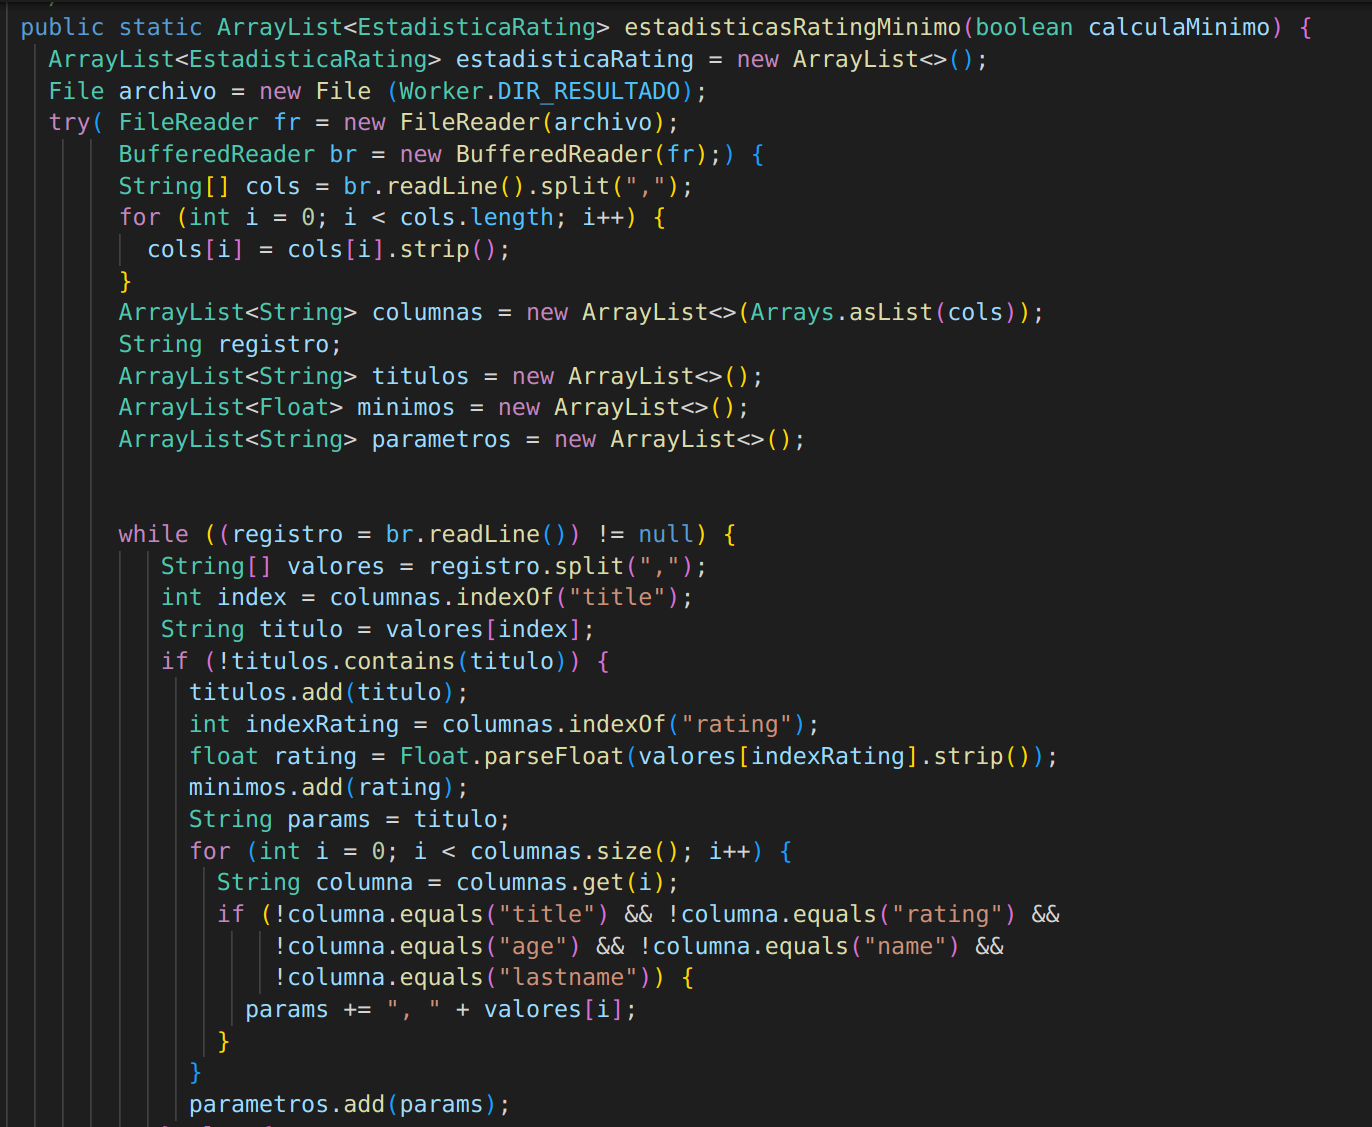
\includegraphics[width=0.9\linewidth]{generaestadisticas_estadisticasratingminimo1}
\end{frame}

% 36
\begin{frame}
\frametitle{GeneraEstadisticas.estadisticasRatingMinimo}
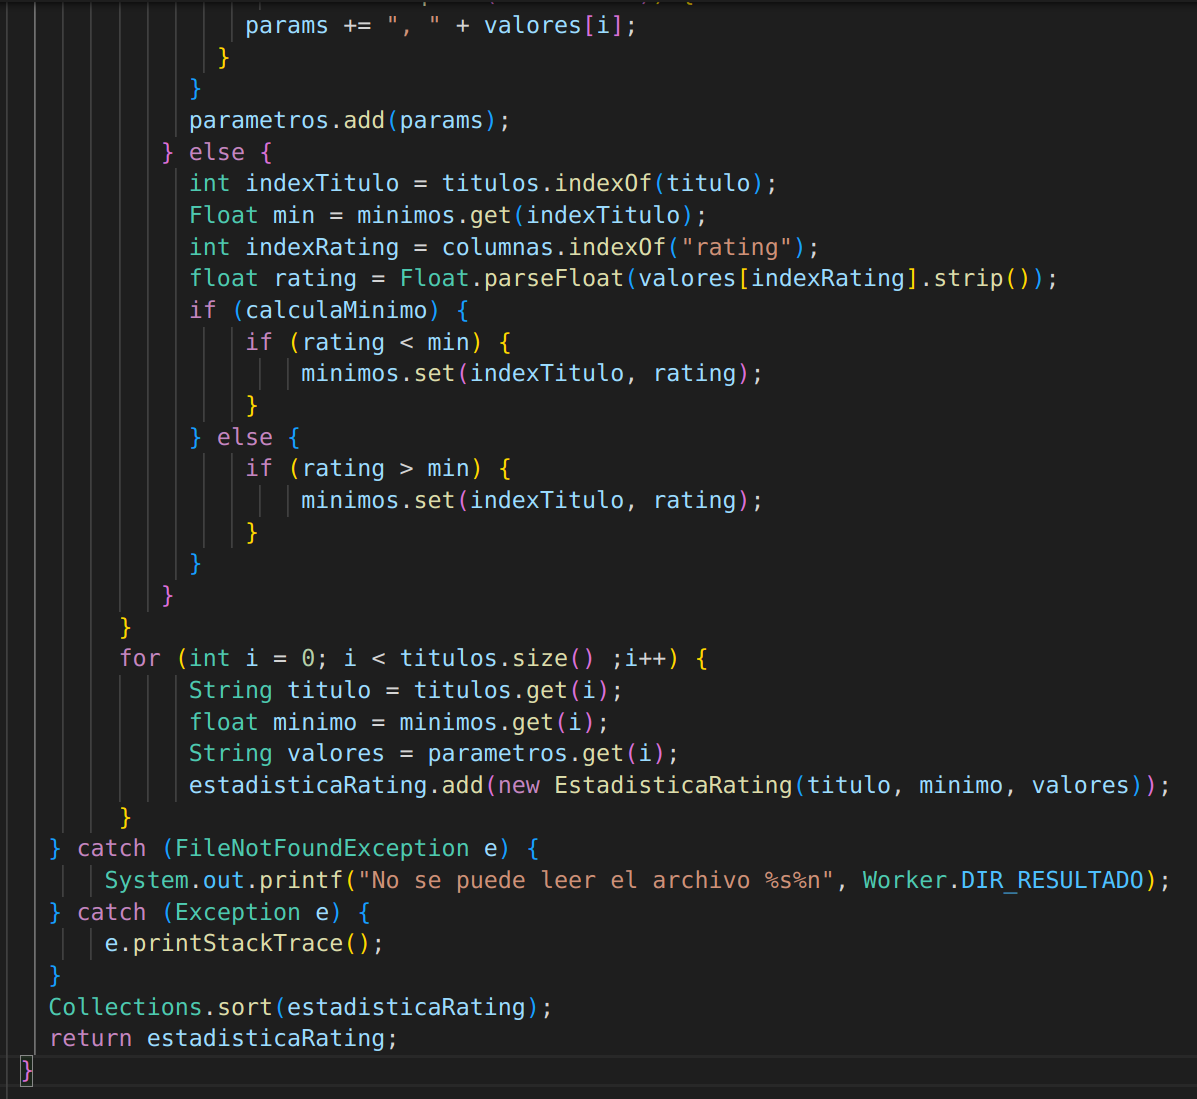
\includegraphics[width=0.9\linewidth]{generaestadisticas_estadisticasratingminimo2}
\end{frame}

% 37
\begin{frame}
\frametitle{GeneraEstadisticas.estadisticasRatingMediana}
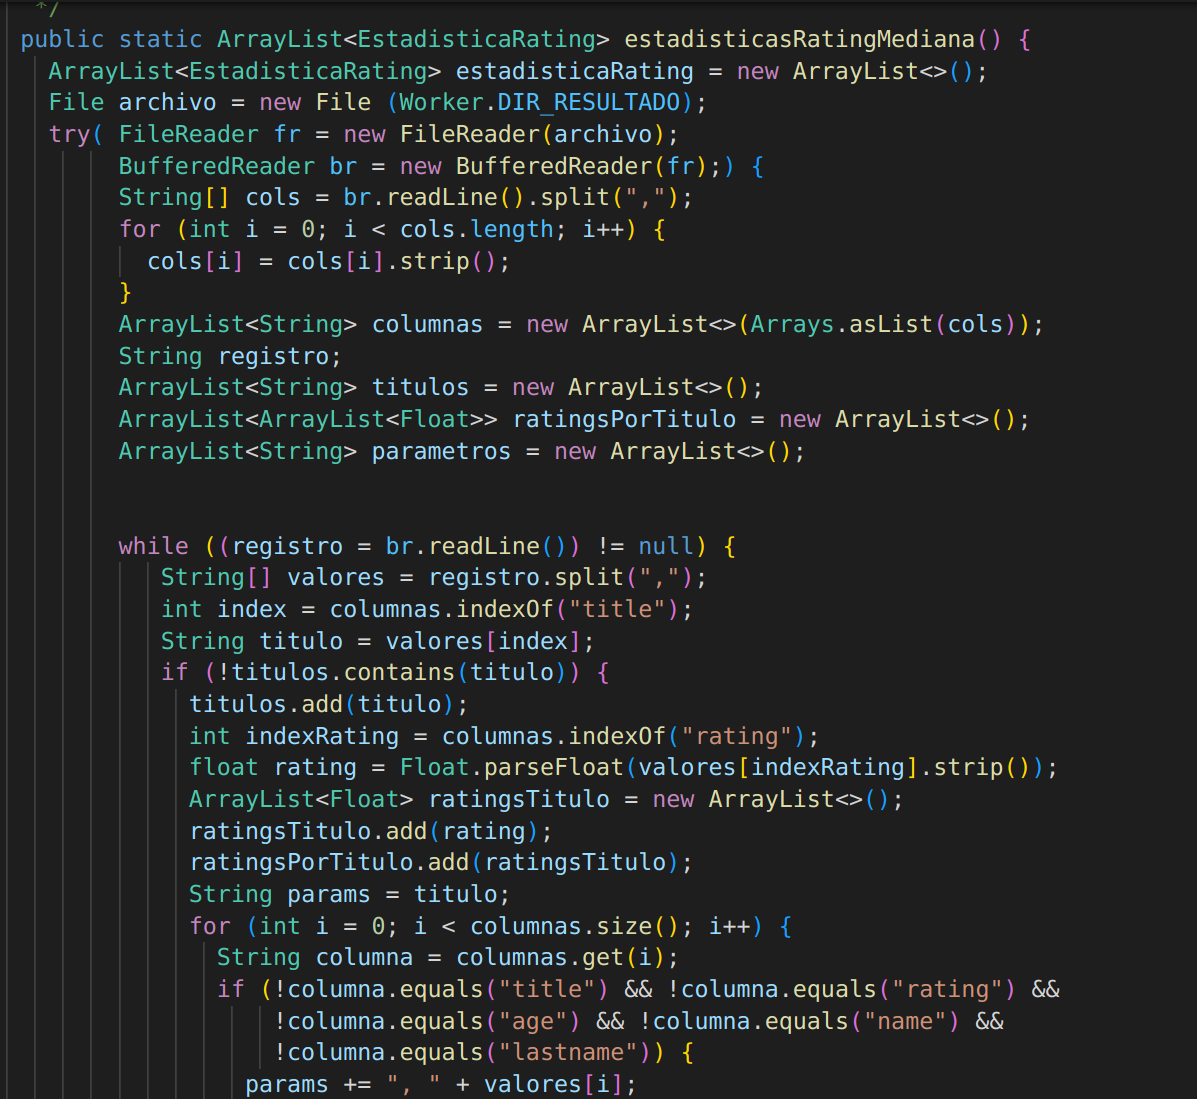
\includegraphics[width=0.9\linewidth]{generaestadisticas_estadisticasratingmediana1}
\end{frame}

% 38
\begin{frame}
\frametitle{GeneraEstadisticas.estadisticasRatingMediana}
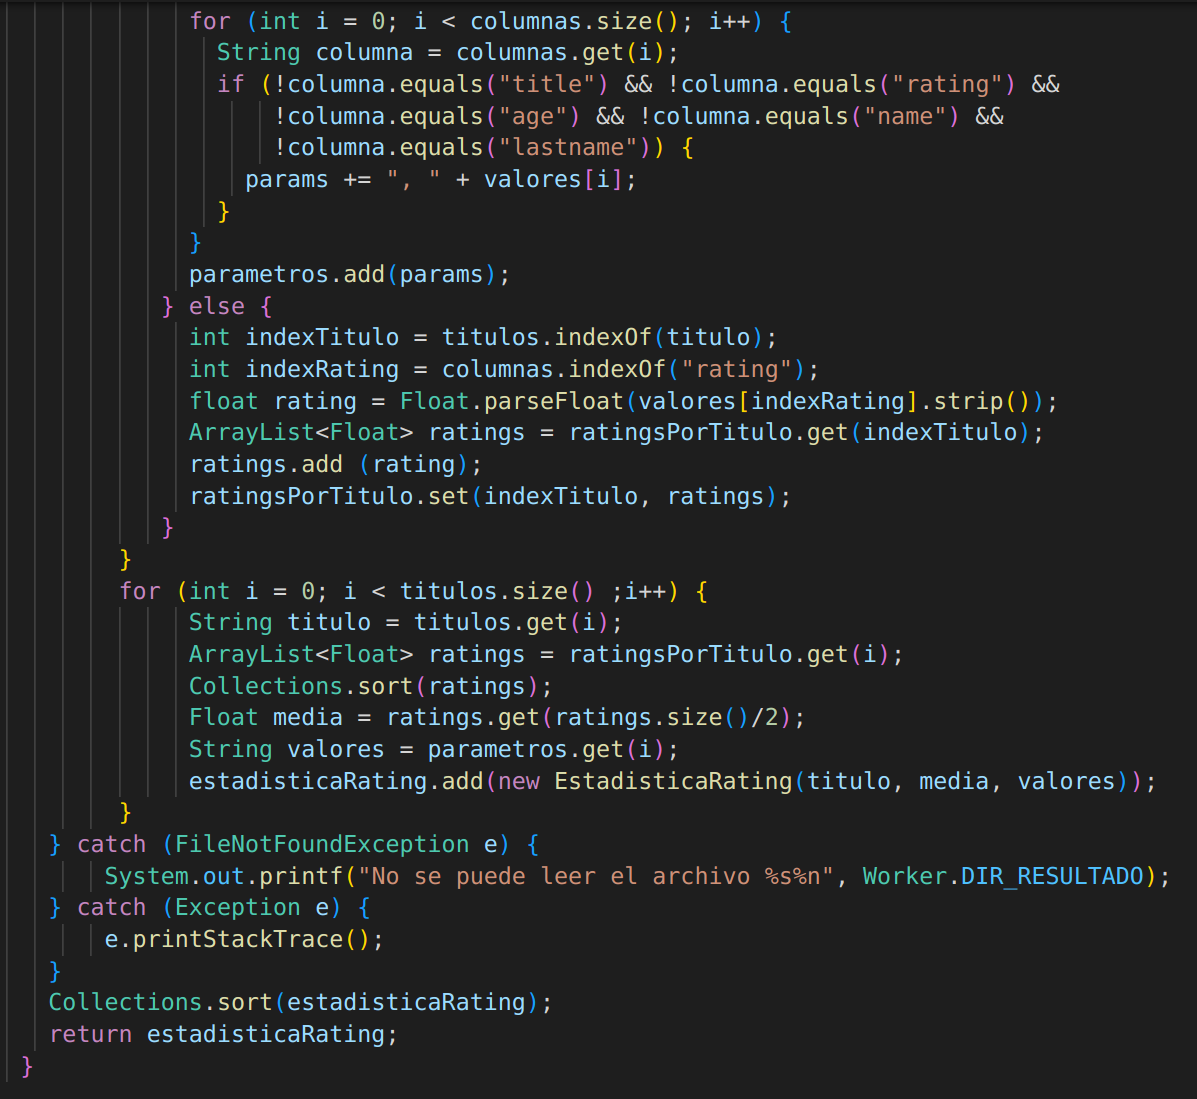
\includegraphics[width=0.9\linewidth]{generaestadisticas_estadisticasratingmediana2}
\end{frame}

\section{GraficaBarras}

% 39
\begin{frame}
\frametitle{GraficaBarras.builder}
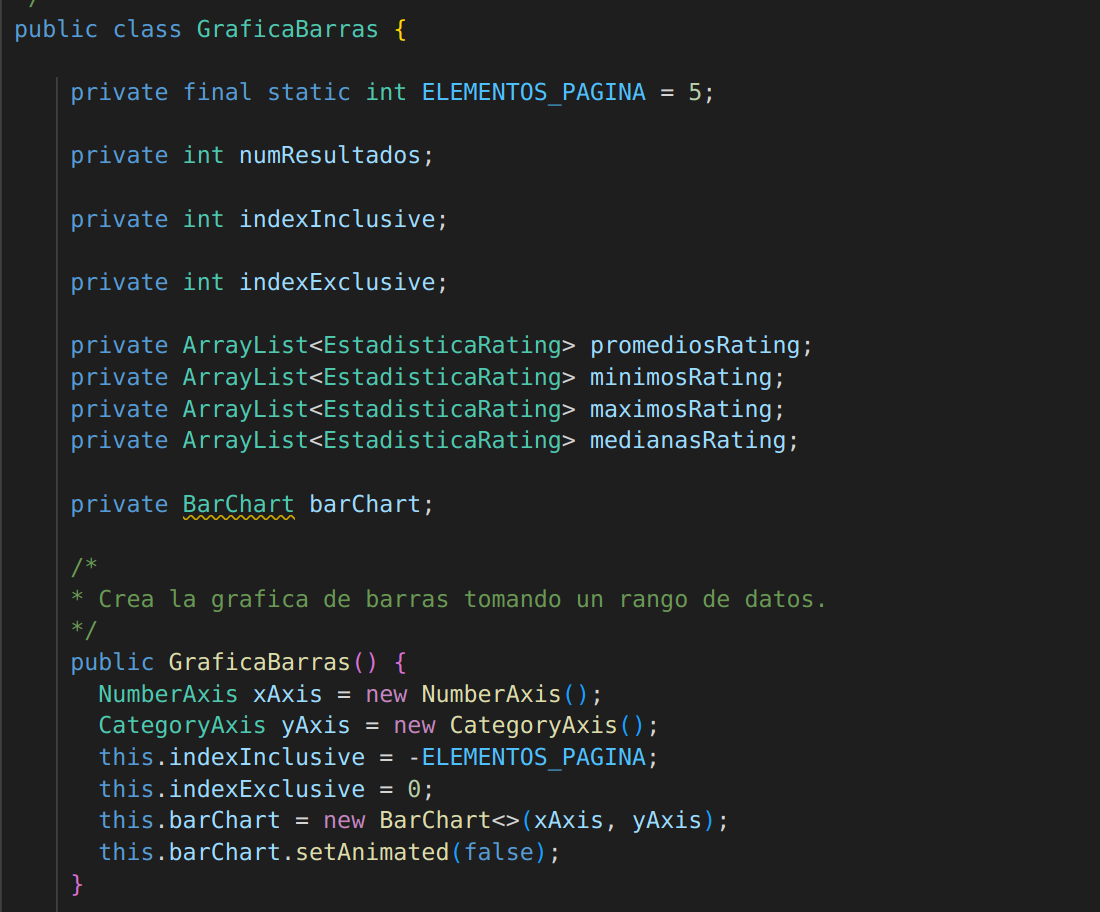
\includegraphics[width=\linewidth]{graficabarras_builder}
\end{frame}

% 40
\begin{frame}
\frametitle{GraficaBarras.avanza}
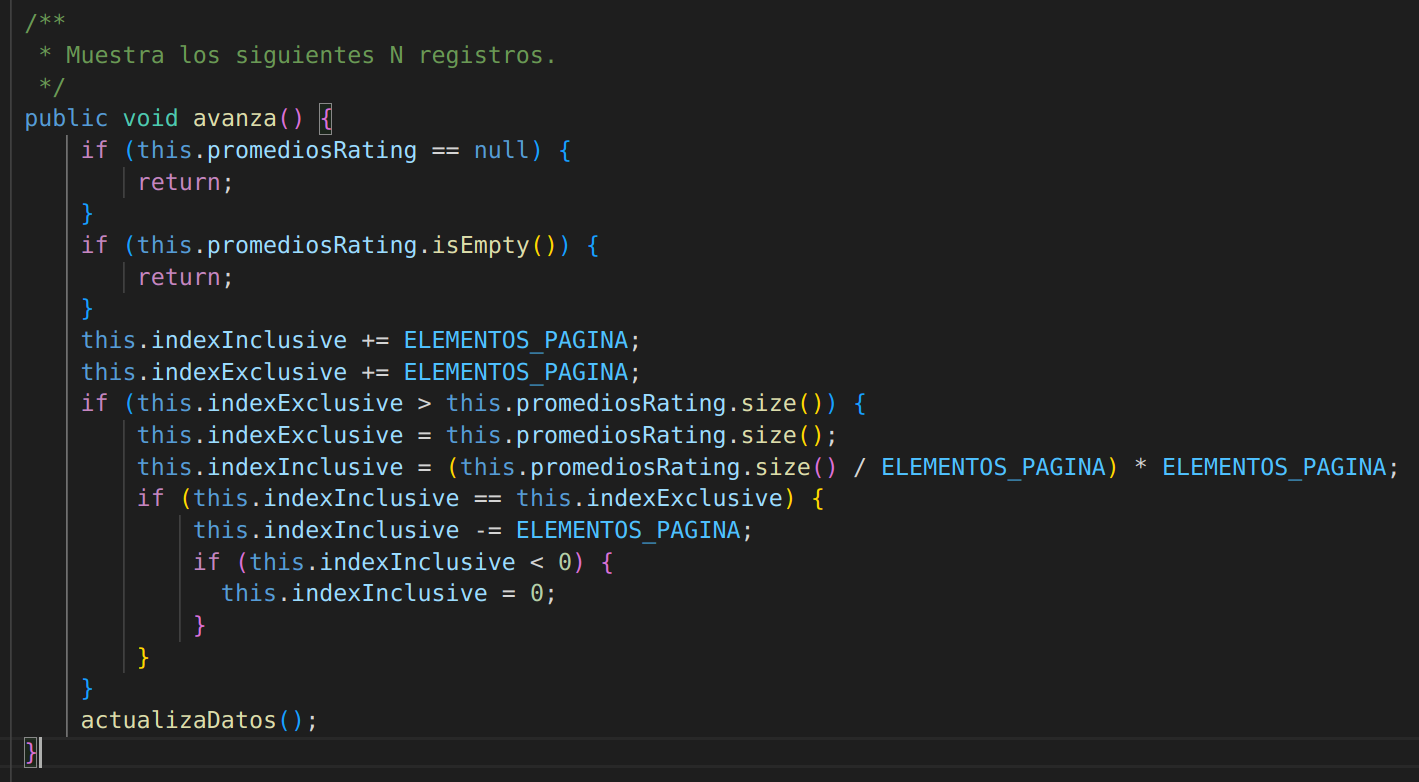
\includegraphics[width=\linewidth]{graficabarras_avanza}
\end{frame}

% 41
\begin{frame}
\frametitle{GraficaBarras.retrocede}
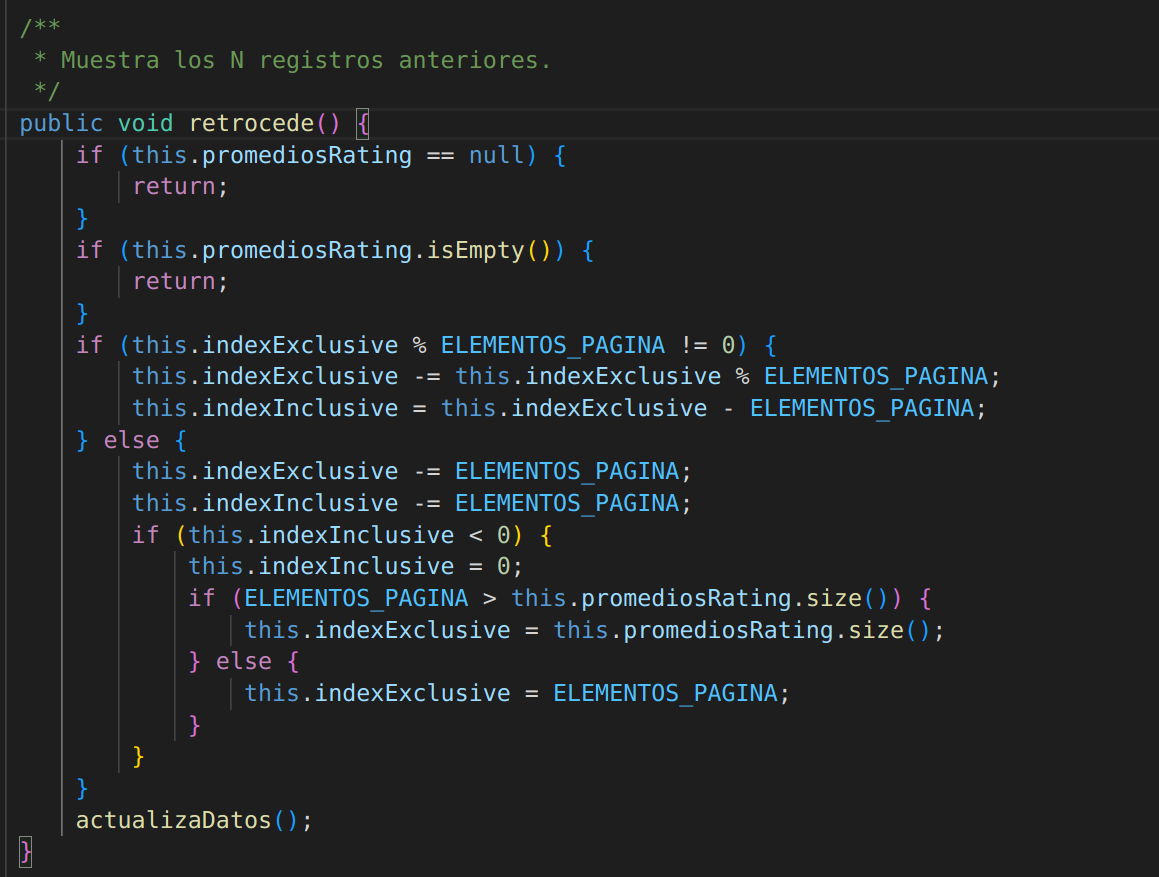
\includegraphics[width=\linewidth]{graficabarras_retrocede}
\end{frame}

% 42
\begin{frame}
\frametitle{GraficaBarras.reset}
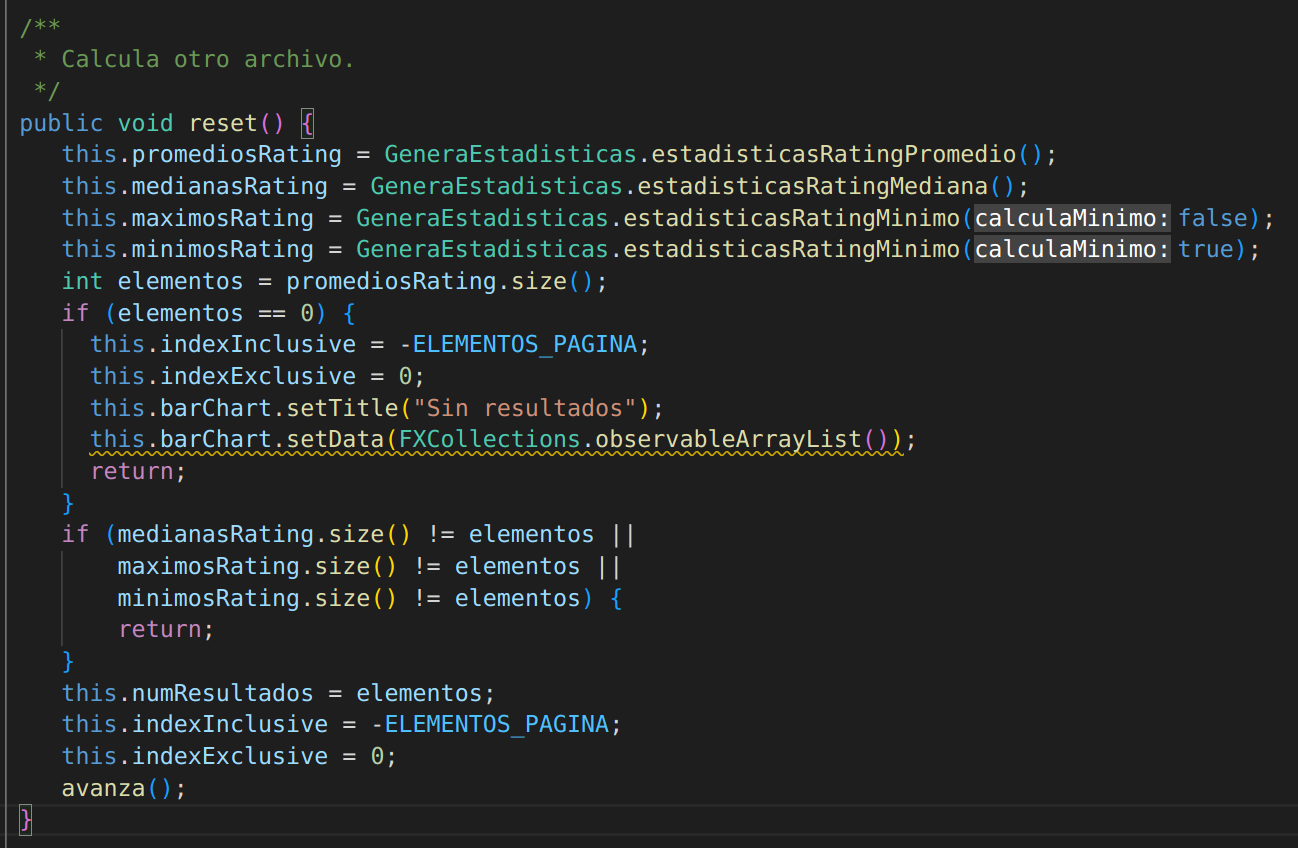
\includegraphics[width=\linewidth]{graficabarras_reset}
\end{frame}

% 43
\begin{frame}
\frametitle{GraficaBarras.obtenDatos}
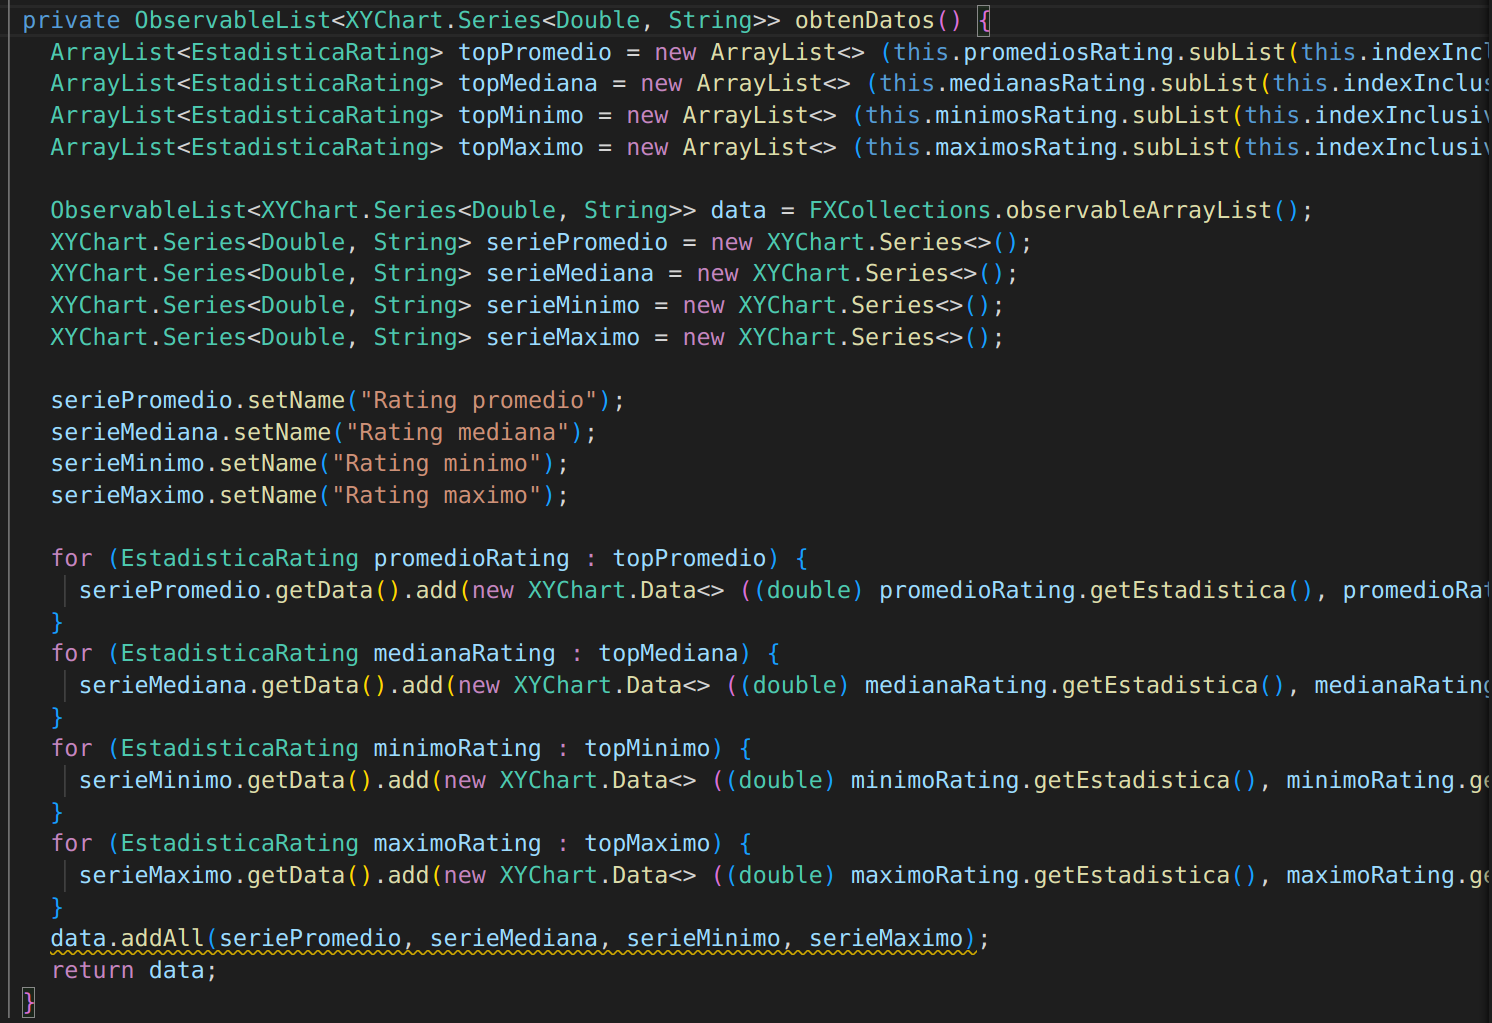
\includegraphics[width=\linewidth]{graficabarras_obtendatos}
\end{frame}

\end{document}

